\documentclass[
    %uninadraft,
    %colorlinks, 
    blacklinks,
    %palatino,
    libertine,
    %mathpazo,
    %tgschola,
    %tgscholamathpazo,
    %alegreya
]{uninathesis}

%\AtBeginDocument{\addtocontents{toc}{\protect\thispagestyle{empty}}} %remove page number from toc

\usepackage[english]{babel}
\addto\captionsenglish{% Replace "english" with the language you use
  \renewcommand{\contentsname}%
    {\sffamily Contents}%
}
\let\openbox\relax
\usepackage{amsthm}
\usepackage{proof}


% Math
\RequirePackage{mathtools}
\RequirePackage{mathrsfs} %need this for mathscr
\let\openbox\relax
\RequirePackage{amsthm}
\RequirePackage{stmaryrd} %for \llbracket

\theoremstyle{plain}
\newtheorem{theorem}{Theorem}

\theoremstyle{definition}
\newtheorem{definition}{Definition}
\newtheorem{example}{Example}

% Tikz - may be removed if unneeded
\RequirePackage{tikz}
\RequirePackage{pgfplots}
\pgfplotsset{compat=1.16}
\usetikzlibrary{positioning,automata,calc,fit,shapes,backgrounds,arrows.meta}
\usepackage{makecell}

% Miscellanea Packages
\RequirePackage[utf8]{inputenc}
\usepackage{ marvosym } %/Lightning
%\usepackage{ stmaryrd } %/lightning
%\usepackage[htt]{hyphenat}
\usepackage{subcaption} %subfigures

% read configuration file
\input{_utils/macro.tex} %can write your macros here

% Bibliography
\RequirePackage{csquotes}
\RequirePackage[sorting=none,maxbibnames=4]{biblatex} %dashed=false to remove dashes on repeated authors.
\bibliography{_bib/bibliography.bib} %bib database(s)

% Front page (package uninafrontespizio)
\Universita{Università degli Studi di Napoli Federico II}
\Facolta{Scuola Politecnica e delle Scienze di Base}
\Dipartimento{Dipartimento di Ingegneria Elettrica e Tecnologie dell'Informazione}
\CorsoDiLaurea{Corso di Laurea Triennale in Informatica}
%\Materia{Verifica di Sistemi}
\AnnoAccademico{2024--2025}
\Titolo{Implementation of a decision procedure for the fluted fragment in Vampire}
\Relatore{Prof.\ Fabio \textsc{Mogavero}}
\Relatore{Prof.\ Massimo \textsc{Benerecetti}}
% \Relatore{Baronessa Filiguelli \textsc{de Bonchamps}}
\RelatoreLabel{Relatori}
\CorrelatoreLabel{}
\Candidato{Riccardo \textsc{Elena}}
\Matricola{N86/4490}
\Logo{logo-federico-II.pdf}
\LogoWidth{3.5cm}
\LogoPosition{below-uni}

%custom hyphenation
\hyphenation{ERTMS/ETCS}

% Theorem-like environments

\newtheorem{lemma}{Lemma}     % Shares numbering with theorems
\newtheorem{proposition}{Proposition}

% Optional: definitions and remarks with different style

\theoremstyle{remark}
\newtheorem{remark}[theorem]{Remark}

% ------------------------------------------------------------------------------------
% Thesis specific custom commands

\usepackage{csvsimple}
\usepackage{longtable}
\usepackage{multicol}

\graphicspath{{_figures/}}
\newcommand{\landor}{\mathrel{\land\mkern-3mu\lor}}
\newcommand{\ms}{\,}
\newcommand{\bold}[1]{\textbf{#1}}
\newcommand{\code}[1]{\lstinline{#1}}
\NewDocumentCommand{\var}{m}{\text{var} (#1)}
\NewDocumentCommand{\flseq}{o m o}{(\overline{\IfValueTF{#1}{#1}{u}}_{#2}\IfValueTF{#3}{,#3}{})}
\NewDocumentCommand{\fldef}{m o m}{\text{Def}_{#1}\IfValueTF{#2}{^{#2}}{}(#3)} %chktex 36

\tikzset{
    syntree/.style={
        level distance=1.5cm,
        sibling distance=2.5cm,
        grow=down,
        % Stile per quantificatori (rettangolare)
        quantifier/.style={draw, rectangle, align=center, 
                           minimum width=1cm, minimum height=0.5cm, 
                           inner sep=2pt},
        % Stile per connettivi (diamond/rombo)
        connective/.style={draw, diamond, align=center, 
                          minimum width=1cm, minimum height=0.4cm,
                          inner sep=1pt},
        % Stile per literal/predicati (ellisse)
        literal/.style={draw, ellipse, align=center, 
                       minimum width=1cm, minimum height=0.4cm,
                       inner sep=1pt}
    }
}

\algnewcommand\algorithmicswitch{\textbf{switch}}
\algnewcommand\algorithmiccase{\textbf{case}}
\algnewcommand\algorithmicdefault{\textbf{default}}

\algdef{SE}[SWITCH]{Switch}{EndSwitch}[1]{\algorithmicswitch\ #1\ \algorithmicdo}{\algorithmicend\ \algorithmicswitch}%
\algdef{SE}[CASE]{Case}{EndCase}[1]{\algorithmiccase\ #1}{\algorithmicend\ \algorithmiccase}%
\algdef{SE}[DEFAULT]{Default}{EndDefault}{\algorithmicdefault}{\algorithmicend\ \algorithmicdefault}%



% -------------------------------------------------------------------------------------------------------

\usepackage[title,titletoc]{appendix}

\begin{document}

    \pagestyle{empty}
    \frontmatter
    \makefrontespizio~\clearpage
    \makefrontespizioalt~\clearpage

    \pagestyle{backmatter}
    \chapter*{Abstract}

First-order logic is undecidable, but several decidable fragments have been identified that retain useful expressive power while guaranteeing termination. The fluted fragment is one such subset, characterized by specific variable ordering constraints in quantified formulae.

This thesis implements and evaluates a decision procedure for the fluted fragment within the Vampire theorem prover. The implementation required three main components: a preprocessing stage that transforms input formulae into the required fluted clause form through structural naming, an adapted literal selection strategy compatible with fluted resolution, and a separation inference rule for handling non-strongly fluted clauses applying dynamic renaming.

The experimental evaluation used both existing TPTP benchmark problems and a custom test generator producing 15,000 synthetic problems. While only 151 naturally occurring fluted problems were found in TPTP, testing revealed that the fluted implementation often matches or outperforms standard Vampire resolution on these problems. The synthetic benchmarks provided more extensive evaluation, showing that specialized preprocessing optimizations can benefit performance even when falling back to standard resolution techniques.

The work demonstrates that implementing decision procedures for specific fragments within general-purpose theorem provers is feasible and can provide computational advantages by exploiting structural properties of the input problems.

% \chapter*{Sommario}
% Qui puoi inserire il sommario (la traduzione dell'abstract in italiano).
% \blindtext[2]
    
    \clearpage
    \tableofcontents

    \mainmatter{}

    \newpage\pagestyle{introduction}

% The \unnumberedchapter, \unnumberedsection commands provided by the uninathesis 
% documentclass add an unnumbered entry to the TOC.
% If you use the starred version of classic sectioning commands (e.g. \chapter*)
% no TOC entry will be added!

\chapter*{Introduction}
% \unnumberedsection{A first unnumbered section}

First-Order Logic (FOL) emerged from the mathematical foundations laid in \textit{Begriffsschrift}~\cite{frege1879} by \citeauthor{frege1879} and in \textit{Principia Mathematica}~\cite{russell1910} by \citeauthor{russell1910}, and has since become a cornerstone formalism in computer science.
Its formal yet expressive nature makes it particularly well-suited for computational reasoning across diverse domains.
In knowledge representation, FOL underpins semantic web technologies and ontology languages like OWL, enabling machines to reason about complex relationships in data.
Meanwhile, in verification, it serves as the logical foundation for model checkers and theorem provers that ensure software correctness, while in artificial intelligence, it historically powered automated reasoning systems and planning algorithms, though modern AI has largely shifted toward statistical and neural approaches that often lack the transparency and formal guarantees that FOL-based systems provide.

However, the expressive power of first-order logic (FOL) comes at a cost: undecidability.
This was established independently in the 1930s by \citeauthor{church1936}~\cite{church1936} using the lambda calculus, and by \citeauthor{turing1936}~\cite{turing1936} via Turing machines---two distinct formalisms that captured the limits of computation.
Their results demonstrated that no algorithm can, in general, determine whether an arbitrary FOL formula is valid. This fundamental limitation creates a significant computational barrier for automated reasoning.
In response, two complementary research directions have emerged: the systematic identification of decidable fragments that retain sufficient expressiveness for practical applications, and the development of automated theorem provers (ATPs) that---while unable to guarantee termination on all inputs---employ sophisticated heuristics and optimizations to solve many real-world problems efficiently.

Among the most prominent automated theorem provers (ATPs) for first-order logic is \textit{Vampire}~\cite{kovacs2013vampire}, a high-performance prover built on advanced saturation-based reasoning.
Vampire combines ordered resolution with literal selection, term indexing, and clause simplification techniques to explore the space of logical consequences efficiently.
It also incorporates modern enhancements such as efficient preprocessing, strategy scheduling, and support for first-order logic with built-in theories.
These features have made Vampire highly successful in competitive settings like the CASC competition, and effective in practical applications ranging from formal verification to software analysis.
Moreover, Vampire's extensible architecture and open-source nature make it the go-to choice for research and experimentation in the field of automated reasoning.

Among the various decidable fragments of FOL, the Fluted Fragment stands out due to its syntactic constraints that preserve decidability while maintaining expressive power in certain contexts. Despite its theoretical appeal, practical tools often do not take advantage of its structural properties.
\uninatodo{Add some references to the Fluted Fragment and some of its applications}

Automated theorem provers (ATPs) such as Vampire employ saturation-based reasoning techniques to handle general FOL problems. While powerful, such tools are often designed to address the full scope of FOL, and do not exploit the structural properties of specific fragments like the Fluted Fragment.

% TODO, put emphasis on th efact that is the problem to be undecidable, and not the specific implementation. 
Moreover, while general-purpose automated theorem provers aim to be as broadly applicable as possible, their completeness comes at the cost of decidability. Since FOL is undecidable in general, such systems may fail to terminate even when the input formula belongs to a decidable fragment. As a result, problems that are in principle solvable — such as those within the Fluted Fragment — may be left unresolved by these tools. In contrast, a specialized decision procedure tailored to the structural constraints of the fragment can guarantee termination and correctness, providing reliable answers where general approaches might not.

This thesis presents the implementation of a saturation-based decision algorithm tailored specifically for the Fluted Fragment. By incorporating structural constraints into the reasoning process, the algorithm aims to provide more efficient decision procedures than general-purpose systems. The performance of the implementation is empirically compared to Vampire to assess the benefits of fragment-specific optimization.
% TODO: add paragraphs about your work

This is the introduction to your work.
\blindtext[3]

\unnumberedsection{Another unnumbered section}

\blindtext[3]

\unnumberedsection{About this thesis work}

Thesis structure, etc.


    \newpage\pagestyle{main}

    \chapter{First Order Logic}\label{chap:first-order-logic}

%\inlineminitoc{}

\noindent First-order logic (FOL), or predicate logic, is a formal system used in mathematics, philosophy, linguistics, and computer science to express statements about objects and their relationships.
It uses \bold{terms} for the representation of objects in the domain of discourse and \bold{predicates} to express properties of these objects or relationships between them.
Moreover, FOL allows for the use of \bold{quantifiers} to make statements that apply to all objects (universal quantification) or some objects (existential quantification) in the domain, and \bold{logical connectives} to construct more complex statements.

One well-known informal statement, \dquote{All humans are mortal} for example, can be expressed in FOL as:
\begin{equation*}
    \forall x \left( \text{H}(x) \implies \text{M}(x) \right)
\end{equation*}

Syntactically speaking, this sentence is composed of:
\begin{itemize}
    \item a \bold{quantifier} \(\forall\)
    \item a \bold{variable} \(x\) which ranges over the whole domain of discourse (possibly every object in the universe)
    \item a \bold{unary predicate} \(\text{H}\) applied to \(x\)
    \item a \bold{unary predicate} \(\text{M}\) applied to \(x\)
    \item a \bold{logical connective} \(\implies\)
\end{itemize}

Upon this syntactic structure, we can build a semantic interpretation, which assigns meaning to the symbols used in the sentence.
In this case, we can interpret \(\text{H}(x)\) as \dquote{\(x\) is a human} and \(\text{M}(x)\) as \dquote{\(x\) is mortal}.
Moreover, the universal quantifier \(\forall\) indicates that the statement applies to all objects in the domain of discourse.
The connective \(\implies\) is the \emph{material implication} of \emph{propositional logic}, indicating that if the first part is true, then the second part must also be true.

As we can see, using FOL we can divide the statement into its syntactic and semantic components, which allows us to reason about its structure separately from its meaning.
This separation permits us to generalize the reasoning process to other syntactically similar statements and to deduce new statements solely from their structure.
This makes FOL particularly suitable for computational treatment: automated systems can manipulate the syntactic form of statements while guaranteeing that these manipulations reflect valid semantic consequences in all interpretations — a property known as \emph{soundness}~\cite{enderton2001}.
As we will see later, this clear separation is crucial for the development of automated reasoning systems, such as the Vampire theorem prover, because it allows us to convert the reasoning task into a syntactic manipulation task, treating statements as symbolic strings with a specific syntax, without the need to explicitly encode the meaning of each statement.

In order to preserve the truth value of statements during this manipulation process, we cannot rely on the syntactic structure alone; we must define a set of rules that act only on the syntactic structure while ensuring truth preservation.
This set of rules is called \bold{inference rules}, and they allow us to derive new statements from existing ones without altering their truth value.
A full exploration of these rules, which form the core of automated reasoning, is reserved for a later chapter. However, a simple example is the well-known rule of \emph{Modus Ponens}, which states that if we know that both \(A\) and \(A\implies B\) are true, then we can conclude \(B\). This illustrates how a new truth can be derived purely from the syntactic form of existing statements.

\section{From Terms to Sentences}\label{sec:from-terms-to-sentences}

First and foremost, we need to rigorously define the structure of first-order logic.
The most basic building blocks of FOL are \bold{terms}, which represent objects in the domain of discourse.
Those are variables (\(x,y,z\)), functions (\(f,g,h\)) and constants (\(a,b,c\)), sometimes viewed as function symbols with arity 0.
Variables are placeholders that can represent any object in the domain, while constants refer to specific objects. Functions map objects to other objects, allowing for more complex expressions.

Terms alone do not constitute statements in FOL, as they lack an associated \emph{truth value}.
The main focus of FOL is on \bold{predicates} (\(P,Q,R\)) ---so the name \emph{predicate logic}---, which are used to express properties of objects or relationships between them.
Examples of predicates include \(\text{H}(x)\) for \dquote{is a human} or \(\text{M}(x)\) for \dquote{is mortal}.
Predicates are applied to terms to form \bold{atomic formulae} (\(A,B\)), the basic units of meaning in FOL\@. They serve as the building blocks of more complex and structured statements, called \bold{formulae} \(\phi, \psi\), obtained by combining atomic formulae using logical connectives and quantifiers.

Solely, not even atomic formulae always bear a truth value, as they can contain \emph{free variables}, namely variables that are not bound by a quantifier. These variables do not refer to any specific object in the domain, and thus the truth value of the atomic formula depends on the interpretation of these variables.
This ambiguity can be illustrated with natural language; for instance, the statement \dquote{X is a human} does not clearly state \emph{which} object \(X\) has to be a human to make the statement true.
The quantifiers resolve this ambiguity by specifying the scope of the variable \(X\). Indeed, the statement \dquote{For all X, X is a human} clearly has a truth value, as it asserts something about every object, whether it is true or not.
Only (atomic) formulae with all variables bound can be said to have a definite truth value, and those are called (\bold{atomic}) \bold{sentences}.

Last but not least, to combine (atomic) formulae/sentences into more complex expressions, we can use logical connectives. Those are symbols that applied to one or more formulae yield a new formula, whose truth value depends on the truth values of the original formulae and on the semantics of the connective.
In particular, the principal connectives used in FOL are:

\begin{itemize}
  \item \bold{Negation} (\(\neg\)): This connective takes a single formula and \bold{inverts} its truth value.
  \item \bold{Conjunction} (\(\land\)): This connective combines two formulae and is \bold{true} if both are true.
  \item \bold{Disjunction} (\(\lor\)): This connective combines two formulae and is \bold{true} if at least one is true.
  \item \bold{Implication} (\(\implies\)): This connective expresses a conditional relationship between two formulae. The new formula is \bold{false} only if the first formula is true and the second formula is false.
  \item \bold{Biconditional} (\(\iff\)): This connective expresses an equivalence between two formulae. The new formula is \bold{true} if both formulae have the same truth value.
\end{itemize}

Commonly, we refer as \emph{literals} to atomic formulae or their negations.
\subsection{Syntax}\label{subsec:syntax}

The syntax of FOL formulae can be formalized with a \emph{context free grammar} (CFG).
In particular, being \(\mathcal{X}\) the set of all variables, \(\mathcal{C}\) the set of all constants, \(\mathcal{F}\) the set of all function symbols, \(\mathcal{P}\) the set of all predicate symbols, we can define the grammar as follows:

\begin{equation}
  FOL = \left( V , \Sigma, \phi \in V, R\right)
\end{equation}
where:
\begin{itemize}
  \item \(V = \{\tau, \alpha, \phi\}\)
  \item \(\Sigma = \mathcal{X} \cup \mathcal{C} \cup \mathcal{F} \cup \mathcal{P} \cup \{\forall, \exists, \land, \lor, \neg, \implies, \iff, \left(,\right), \top, \bot\}\)
   \item \(R\) = \begin{flalign}
    \begin{aligned}
      \tau \rightarrow  \ms  &x \in \mathcal{X}  \ms | \ms  
                        c \in \mathcal{C}  \ms | \ms  
                        f(\tau,\ldots,\tau) \in \mathcal{F} \\
      \alpha \rightarrow  \ms  &P(\tau,\ldots,\tau), P \in \mathcal{P} \\
      \phi \rightarrow  \ms  &\alpha  \ms | \ms  \top  \ms | \ms  \bot  \ms | \ms  
       \neg\phi  \ms |
       \left(\phi\land\phi\right) |
       \left(\phi\lor\phi\right) |
       \left(\phi\implies\phi\right) |
       \left(\phi\iff\phi\right) |  \ms 
       \forall x\left(\phi\right)  \ms | \ms 
       \exists x\left(\phi\right)
    \end{aligned} &&
  \end{flalign}
\end{itemize}

The language generated by this grammar is the set of all \emph{well-formed formulae} in FOL\@.
Every string of the so generated language can also be represented with a \emph{syntactic tree}, which is a tree representation of the syntactic structure of the formula, highlighting the hierarchical relationships between its components.
An example of a syntactic tree for the formula \(\forall x \left(\text{H}(x) \implies \text{M}(x)\right)\) is shown in Figure~\ref{fig:syntactic_tree}.

\begin{figure}[H]
    \centering
    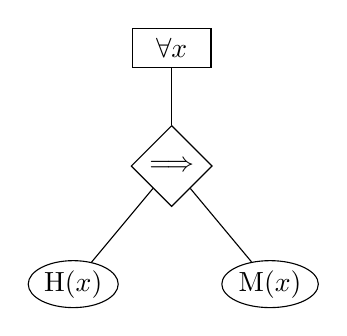
\begin{tikzpicture}[syntree]
        \node[quantifier] {{\(\forall x\)}}
            child { node[connective] {\(\implies\)} 
              child { node[literal] {\(\text{H}(x)\)} }
              child { node[literal] {\(\text{M}(x)\)} }
            };
    \end{tikzpicture}
    \caption{Syntactic tree for \(\forall x (\text{H}(x) \implies \text{M}(x))\)}\label{fig:syntactic_tree}
\end{figure}

In this representation, it is possible to omit the parentheses around the subformulae, as the tree structure already encodes the necessary grouping.
For the sake of brevity, in formulae tree representations, atoms will be represented collapsed into single nodes, as shown in the example above.
Moreover, is possible to isolate a \emph{subgrammar} by considering only the rules that generate atomic formulae (excluding so the ones deriving from \(\phi\)). Doing this easily allows to define the concept of \bold{subterm} as a \emph{proper subtree} of the syntactic tree that represents an atomic formula.
An example of such a tree is shown in Figure~\ref{fig:subterm_tree} for the atomic formula \(P(f(x, g(y)))\).
\begin{figure}[H]
    \centering
    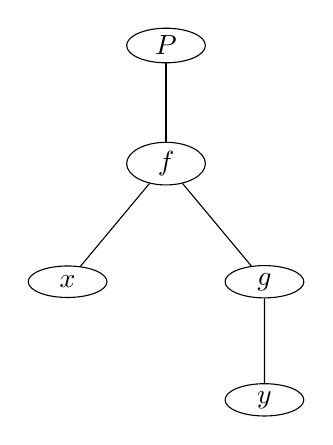
\begin{tikzpicture}[syntree]
        \node[literal] {\(P\)}
            child { node[literal] {\(f\)}
              child { node[literal] {\(x\)} }
              child { node[literal] {\(g\)}
                child { node[literal] {\(y\)} }
              }
            };
    \end{tikzpicture}
    \caption{Syntactic tree for the atomic formula \(P(f(x, g(y)))\) showing nested function structure}\label{fig:subterm_tree}
\end{figure}

If we consider multiple atomic formulae, is possible to represent them as a \bold{forest} of syntactic trees, where each tree represents an atomic formula.

\begin{figure}[H]
    \centering
    \begin{minipage}[t]{0.48\textwidth}
        \centering
        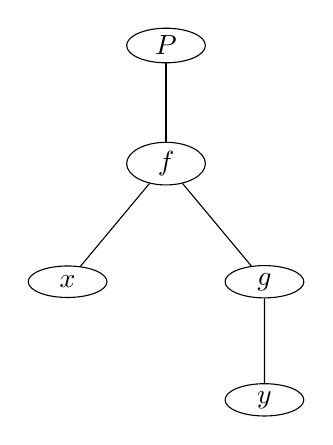
\begin{tikzpicture}[syntree]
            \node[literal] {\(P\)}
                child { node[literal] {\(f\)}
                  child { node[literal] {\(x\)} }
                  child { node[literal] {\(g\)}
                    child { node[literal] {\(y\)} }
                  }
                };
        \end{tikzpicture}
    \end{minipage}
    \hfill
    \begin{minipage}[t]{0.48\textwidth}
        \centering
        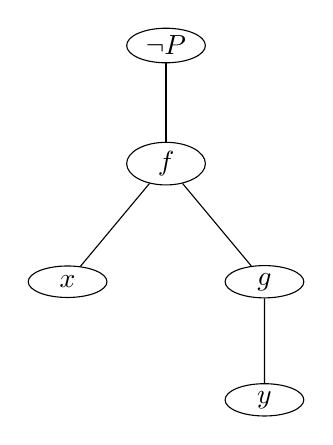
\begin{tikzpicture}[syntree]
            \node[literal] {\(\neg P\)}
                  child { node[literal] {\(f\)}
                    child { node[literal] {\(x\)} }
                    child { node[literal] {\(g\)}
                      child { node[literal] {\(y\)} }
                    }
                  };
        \end{tikzpicture}
    \end{minipage}
    \caption{Forest of the atomic formulae \(P(f(x, g(y)))\) and \(\neg P(f(x, g(y)))\)}\label{fig:subterm_forest}
\end{figure}


In practice, it is often more convenient to represent these structures as Directed Acyclic Graphs (DAGs) rather than trees. This is because DAGs allow for the sharing of subterms, which can lead to more compact representations and easier manipulation of the formulae.
DAGs can be particularly useful in automated reasoning and theorem proving, where the same subterm may appear in multiple places within a formula. By representing the formula as a DAG, we can avoid redundant copies of the subterms and simplify the reasoning process.

\begin{figure}[H]
    \centering
    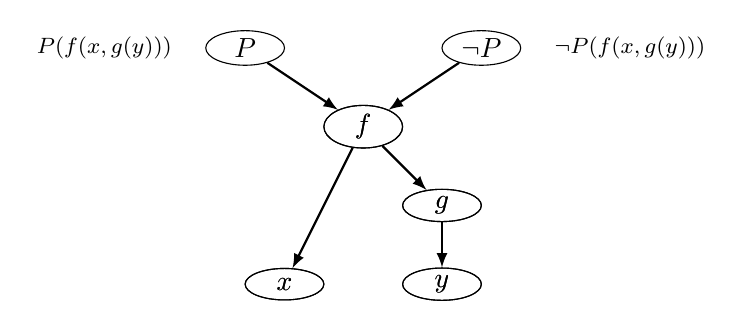
\begin{tikzpicture}[syntree]
        % Livello delle variabili (condivise)
        \node[literal] (x) at (0,0) {\(x\)};
        \node[literal] (y) at (2,0) {\(y\)};
        
        % Livello delle funzioni (condivise)
        \node[literal] (g) at (2,1) {\(g\)};
        \node[literal] (f) at (1,2) {\(f\)};
        
        % Livello dei predicati (separati)
        \node[literal] (P_pos) at (-0.5,3) {\(P\)};
        \node[literal] (P_neg) at (2.5,3) {\(\neg P\)};
        
        % Connessioni condivise
        \draw[-latex, thick] (g) -- (y);
        \draw[-latex, thick] (f) -- (x);
        \draw[-latex, thick] (f) -- (g);

        % Connessioni per literal positivo
        \draw[-latex, thick] (P_pos) -- (f);

        % Connessioni per literal negativo
        \draw[-latex, thick] (P_neg) -- (f);


        % Etichette
        \node[left=0.3cm of P_pos, font=\footnotesize] {\(P(f(x, g(y)))\)};
        \node[right=0.3cm of P_neg, font=\footnotesize] {\(\neg P(f(x, g(y)))\)};
        
        % Evidenzia i nodi condivisi con colore diverso
        \node[literal] at (x) {\(x\)};
        \node[literal] at (y) {\(y\)};
        \node[literal] at (g) {\(g\)};
        \node[literal] at (f) {\(f\)};
    \end{tikzpicture}
    \caption{DAG representation showing shared subterms between \(P(f(x, g(y)))\) and \(\neg P(f(x, g(y)))\)}\label{fig:subterm_dag}
\end{figure}

\subsection{Semantics}\label{subsec:semantics}

To formalize semantics in FOL, we need to define the meaning of the symbols and the truth conditions for the formulae. This is typically done using a \emph{model}, which consists of a domain of discourse and an interpretation function that assigns meanings to the constants, functions, and predicates.

A \bold{model} for a FOL language is a pair \(M = (D, I)\), where:
\begin{itemize}
  \item \(D\) is a non-empty set, called the \bold{domain of discourse}.
  \item \(I\) is an interpretation function that assigns:
  \begin{itemize}
    \item Each constant \(c \in \mathcal{C}\) to an element \(I(c) \in D\).
    \item Each function symbol \(f \in \mathcal{F}\) to a function \(I(f): D^{n_f} \to D\), where \(n_f\) is the arity of \(f\).
    \item Each predicate symbol \(P \in \mathcal{P}\) to a relation \(I(P) \subseteq D^{n_P}\), where \(n_P\) is the arity of \(P\).
  \end{itemize}
\end{itemize}
The truth value of a formula \(\phi\) in a model \(M\) is determined by the interpretation function and the structure of the formula as follows:

\subsubsection{Variable Assignment}\label{subsubsec:variable_assignment}
Given a model \(M = (D, I)\), a \bold{variable assignment} (or \bold{valuation}) is a function \(\sigma: \mathcal{X} \to D\) that assigns each variable to an element of the domain. We denote by \(\sigma[x \mapsto d]\) the assignment that is identical to \(\sigma\) except that it maps variable \(x\) to element \(d \in D\).

\subsubsection{Term Evaluation}\label{subsubsec:term_evaluation}
The \bold{evaluation} of a term \(t\) in model \(M\) under assignment \(\sigma\), denoted \(\llbracket t \rrbracket_M^\sigma\), is defined recursively:
\begin{itemize}
  \item If \(t\) is a variable \(x\), then \(\llbracket x \rrbracket_M^\sigma = \sigma(x)\).
  \item If \(t\) is a constant \(c\), then \(\llbracket c \rrbracket_M^\sigma = I(c)\).
  \item If \(t = f(t_1, \ldots, t_n)\) where \(f\) is an \(n\)-ary function symbol, then 
        \[\llbracket f(t_1, \ldots, t_n) \rrbracket_M^\sigma = I(f)(\llbracket t_1 \rrbracket_M^\sigma, \ldots, \llbracket t_n \rrbracket_M^\sigma)\]
\end{itemize}

\subsubsection{Truth Conditions}\label{subsubsec:truth_conditions}
The \bold{satisfaction} of a formula \(\phi\) in model \(M\) under assignment \(\sigma\), denoted \(M, \sigma \models \phi\), is defined recursively:

\begin{itemize}
  \item \bold{Atomic formulae:}
  \begin{itemize}
    \item \(M, \sigma \models P(t_1, \ldots, t_n) \leftrightarrow (\llbracket t_1 \rrbracket_M^\sigma, \ldots, \llbracket t_n \rrbracket_M^\sigma) \in I(P)\)
    \item \(M, \sigma \models \top\) (always true)
    \item \(M, \sigma \not\models \bot\) (never true)
  \end{itemize}
  
  \item \bold{Logical connectives:}
  \begin{itemize}
    \item \(M, \sigma \models \neg \phi \leftrightarrow M, \sigma \not\models \phi\)
    \item \(M, \sigma \models \phi \land \psi \leftrightarrow M, \sigma \models \phi\) and \(M, \sigma \models \psi\)
    \item \(M, \sigma \models \phi \lor \psi \leftrightarrow M, \sigma \models \phi\) or \(M, \sigma \models \psi\)
    \item \(M, \sigma \models \phi \implies \psi \leftrightarrow M, \sigma \not\models \phi\) or \(M, \sigma \models \psi\)
    \item \(M, \sigma \models \phi \iff \psi \leftrightarrow \left(M, \sigma \models \phi \text{ and } M, \sigma \models \psi\right) \text{ or } \left(M, \sigma \not\models \phi \text{ and } M, \sigma \not\models \psi\right)\)
  \end{itemize}
  
  \item \bold{Quantifiers:}
  \begin{itemize}
    \item \(M, \sigma \models \forall x  \ms  \phi\) if and only if for all \(d \in D\), \(M, \sigma[x \mapsto d] \models \phi\)
    \item \(M, \sigma \models \exists x  \ms  \phi\) if and only if there exists some \(d \in D\) such that \(M, \sigma[x \mapsto d] \models \phi\)
  \end{itemize}
\end{itemize}

\subsubsection{Semantic Notions}\label{subsubsec:semantic_notions}
A formula \(\phi\) is:
\begin{itemize}
  \item \bold{Satisfiable} if there exists a model \(M\) and assignment \(\sigma\) such that \(M, \sigma \models \phi\).
  \item \bold{Valid} (sometimes called a \bold{tautology}) if for all models \(M\) and assignments \(\sigma\): \(M, \sigma \models \phi\). We write \(\models \phi\).
  \item \bold{Unsatisfiable} (or \bold{contradictory}) if for all models \(M\) and assignments \(\sigma\): \(M, \sigma \not\models \phi\).
\end{itemize}

For a set of formulae \(\Gamma\) and a formula \(\phi\), we say \(\Gamma\) \bold{semantically entails} \(\phi\), written \(\Gamma \models \phi\), if for all models \(M\) and assignments \(\sigma\):
  \[\text{if } M, \sigma \models \psi \text{ for all } \psi \in \Gamma, \text{ then } M, \sigma \models \phi\]
It is worth noticing that satisfiability and validity are closely related:
\begin{theorem}[Validity-Satisfiability Reduction]\label{thm:validity_satisfiability_reduction}
A formula \(\phi\) is valid if and only if \(\neg\phi\) is unsatisfiable. Formally:
\[\models \phi \iff M,\sigma\not\models\neg\phi \text{, for all } M,\sigma\]
\end{theorem}

\begin{proof}[Proof Sketch]
To prove this theorem, we need to show both directions of the equivalence.
  \begin{description}
    \item[(\(\Rightarrow\))] If \(\phi\) is valid, then \(M, \sigma \models \phi\) for all models \(M\) and assignments \(\sigma\). Therefore, assuming tertium non datur, \(M, \sigma \not\models \neg\phi\) for all \(M, \sigma\), making \(\neg\phi\) unsatisfiable.
    \item[(\(\Leftarrow\))] If \(\neg\phi\) is unsatisfiable, then there is no model \(M\) and assignment \(\sigma\) such that \(M, \sigma \models \neg\phi\). Therefore, for all \(M, \sigma\), again assuming tertium non datur we have \(M, \sigma \models \phi\), making \(\phi\) valid.
  \end{description}
\qed{}
\end{proof}


\section{Substitutions and Unification}\label{sec:substitutions-and-unification}
In Section~\ref{subsubsec:variable_assignment} we introduced the notation \(\sigma[x \mapsto d]\) to indicate a variable assignment in the semantic evaluation of a formula. We now extend this concept to the purely \emph{syntactic} setting, where variables are replaced by \emph{terms} rather than by elements of the interpretation domain. This leads to the notions of \emph{substitution}, \emph{unification}, and \emph{most general unifier}.

\subsection{Substitutions}\label{subsec:substitutions}
Given a term or literal \(\tau\), the notation \(\tau[x_k \mapsto t]\) denotes the expression obtained by replacing every occurrence of the variable \(x_k\) in \(\tau\) with the term \(t\).  
For example, if \(\tau = g(x_1, x_2)\), then:
\begin{equation}
\tau[x_1 \mapsto h] = g(h, x_2)
\end{equation}
A \bold{substitution} is a function mapping a subset of variables \(\mathcal{X}^{'} \subseteq \mathcal{X}\) to a set of terms \(\mathcal{T} \subseteq \mathcal{X} \cup \mathcal{F} \cup \mathcal{C}\):
\begin{equation}
\sigma = \{ x_1\mapsto t_1, \ldots, x_n\mapsto t_n \}
\end{equation}
If \(\tau\) is a term and \(\sigma\) is a substitution, we write \(\tau\sigma\) or \(\tau[x_1 \mapsto t_1, \ldots, x_n \mapsto t_n]\) for the term obtained by replacing all \(x_i\) with \(t_i\) \emph{simultaneously}.  
The word “simultaneously” means that each replacement is made with respect to the \emph{original} \(\tau\), without the effect of one replacement influencing another.

For instance, if \(\tau = f(x_1, x_2)\), then:
\begin{equation}
\tau[x_1 \mapsto x_2,  \ms  x_2 \mapsto x_1] = f(x_2, x_1)
\end{equation}
and not \(f(x_1, x_1)\), which would arise from sequential application.

\subsection{Generality of  Substitutions}\label{subsec:generality-of-substitutions}
For two substitutions \(\sigma_1\) and \(\sigma_2\), we say \(\sigma_1\) is \bold{more general} than \(\sigma_2\) if for every term \(\tau\) there exists a substitution \(\theta\) such that:
\begin{equation}  
  \tau\sigma_2 = (\tau\sigma_1)\theta
\end{equation}
If there is a substitution \(\sigma\) with:
\begin{equation}
\tau_1\sigma = \tau_2\sigma
\end{equation}
then \(\tau_1\) and \(\tau_2\) are said to be \bold{unifiable}, and \(\sigma\) is called a \bold{unifier}.
A unifier \(\sigma\) for two terms \(\tau_1\) and \(\tau_2\) is called the \bold{most general unifier} (MGU) if it is more general than any other unifier of \(\tau_1\) and \(\tau_2\).

\subsection{Unification Beyond Single Terms}\label{subsec:unification-beyond-single-terms}
The unification concept extends to sets of terms, literals, and sets of literals.  
A set of terms \(\mathcal{T}\) is \bold{unifiable} if there exists a substitution \(\sigma\) such that for any \(\tau_i, \tau_j \in \mathcal{T}\) we have \(\tau_i\sigma = \tau_j\sigma\). In this case, \(\sigma\) is a unifier of \(T\).

Two literals with the same arity:
\begin{equation}
L_1 = P(\tau_1, \ldots, \tau_n), \quad L_2 = \neg P(\tau'_1, \ldots, \tau'_n)
\end{equation}
are unifiable if there is a substitution making them identical, disregarding negation.
Literals of different arities are never unifiable.

\subsection{Obstructions to Unification}\label{subsec:obstructions-to-unification}
When attempting to unify two terms, two main forms of obstruction can occur:
\begin{enumerate}
    \item \bold{Function obstruction:} in a parallel traversal of the syntactic trees of both terms, two different function symbols occur at corresponding positions. For example:
    \[
    f(x_1, g_1(x_2)) \quad\text{and}\quad f(x_1, g_2(x_2))
    \]
    are not unifiable because \(g_1 \neq g_2\).
    \item \bold{Variable obstruction:} in a parallel traversal, a variable \(x\) appears in one term while the other term contains a subterm \(t \neq x\) in which \(x\) occurs. For example:
    \[
    h(x_1, k(x_2)) \quad\text{and}\quad h(k(x_1), x_1)
    \]
    are not unifiable because \(x_1\) occurs inside \(k(x_1)\).
\end{enumerate}

In general so, if two terms are not unifiable, then at least one of the following holds:
\begin{enumerate}
    \item The terms have different arities.
    \item The terms exhibit a function obstruction.
    \item The terms exhibit a variable obstruction.
\end{enumerate}


\subsection{Complexity of Unification}\label{subsec:complexity-of-unification}
The computational complexity of unification has been extensively studied since the 1960s.
Early approaches exhibited worst-case exponential behaviour due to the difficulty of detecting variable obstructions efficiently~\cite{robinson1965}.
However, significant theoretical advances in the 1970s led to the development of linear-time unification algorithms that achieve \(O(n)\) complexity, where \(n\) is the combined size of the input terms~\cite{martelli1976, paterson1978}.

These linear-time bounds represent optimal complexity for the unification problem, as any algorithm must examine all symbols in the input terms at least once.
Modern implementations incorporate various optimization techniques such as term indexing and specialized handling for common cases to improve average-case performance~\cite{martelli1976}.
The unification problem belongs to complexity class \bold{P}, making it tractable for practical applications in automated reasoning and logic programming systems.


\section{Skolemization and Normalization}\label{sec:skolemization_and_normalization}

Often times, First-Order formulae undergo a series of transformations to prepare them for automated reasoning tasks.
These transformations include renaming variables, converting to normal forms, and Skolemization.
Raw first-order logic formulae, as naturally expressed, are typically not in a form that automated theorem provers and inference engines can efficiently process.
The transformation process standardizes the syntactic structure of formulae, eliminates certain logical constructs that complicate automated reasoning, and converts them into canonical forms that enable the systematic application of inference rules and resolution procedures.

\subsection{Negated Normal Form}\label{subsec:negated_normal_form}
The first transformation applied is to convert the formula into \bold{negated normal form} (NNF).

A formula is in NNF if it is described by the following CFG\@:
\begin{equation}
  \nu \to \top  \ms | \ms  \bot  \ms | \ms  L  \ms | \ms  \nu \land \nu  \ms | \ms  \nu \lor \nu  \ms | \ms  \forall x  \ms  \nu  \ms | \ms  \exists x  \ms  \nu \quad\quad \text{where } L \text{ is a literal}
\end{equation}
In a practical sense, NNF transformation involves pushing negations inward and eliminating implications and biconditionals.
In fact, every formula can be brought into this form by replacing implications (\(\implies\)) and equivalences (\(\iff\)) by their definitions, using De Morgan's laws to push negation inwards, and eliminating double negations. This process can be represented using the following rewrite rules:

\begin{equation}
  \begin{aligned}
    \phi \implies \psi &\leadsto \neg \phi \lor \psi \\
    \phi \iff \psi &\leadsto (\neg \phi \lor \psi) \land (\phi \lor \neg \psi) \\
    \neg (\phi \lor \psi) &\leadsto \neg \phi \land \neg \psi \\
    \neg (\phi \land \psi) &\leadsto \neg \phi \lor \neg \psi \\
    \neg \neg \phi &\leadsto \phi \\
    \neg \exists x  \ms  \phi &\leadsto \forall x  \ms  \neg \phi \\
    \neg \forall x  \ms  \phi &\leadsto \exists x  \ms  \neg \phi
  \end{aligned}
\end{equation}
The NNF version of a formula is \emph{equivalent} to the original formula, meaning they have the same truth value in every model.

\subsection{Skolemization}\label{subsec:skolemization}
In the context of automated reasoning, \bold{Skolemization} is the process of eliminating existential quantifiers from a formula by introducing new symbols called \bold{Skolem functions} or \bold{Skolem constants}~\cite{skolem1920}.  
The result of Skolemization is not logically equivalent to the original formula but, relying on the axiom of choice, it is \bold{equisatisfiable}: the original formula is satisfiable if and only if the Skolemized version is satisfiable.
The process of Skolemization goes as follows:

Let \(\phi\) be a formula in NNF\@. For every existential quantifier \(\exists x_k\) in \(\phi\):
\begin{itemize}
  \item If \(x_k\) is not in the scope of any universal quantifier, replace it with a new constant symbol \(c\) (a \emph{Skolem constant}).
  \item If \(x_k\) is in the scope of universal quantifiers over variables \(y_1, \dots, y_m\), replace \(x_k\) with a new function symbol \(f(y_1, \dots, y_m)\) (a \emph{Skolem function}) of arity \(m\).
\end{itemize}
All Skolem symbols introduced must be fresh, i.e., not present in the original formulae.
An example of this process is as follows:

Consider the formula:
\[
\forall x \: \exists y \: P(x, y)
\]
Since \(y\) is existentially quantified within the scope of \(\forall x\), we introduce a function \(f(x)\):
\[
\forall x \: P(x, f(x))
\]

The Skolemization process fundamentally transforms the logical structure of a formula completely eliminating all existential quantifiers from it, replacing them with concrete function or constant symbols that capture the dependencies between variables.
As mentioned before though, this transformation preserves satisfiability, but it does not preserve validity in the reverse direction.
A formula that is valid before Skolemization may lose this property afterward, since the introduction of Skolem functions can create additional constraints that were not present in the original formula.
However, the resulting formula contains only universal quantifiers, which significantly simplifies the reasoning process by enabling purely universal reasoning techniques. 
This uniform quantifier structure is especially advantageous for automated theorem provers, as it eliminates the need to handle the complex interactions between universal and existential quantifiers% during proof search.

\subsection{Clausal Normal Form}\label{subsec:clausal_normal_form}
A formula is in CNF if it is a conjunction of one or more \bold{clauses}, each clause being a disjunction of literals.  
As NNF, CNF can be described by a CFG too:
\begin{equation}
  \begin{aligned}
    CNF &\to D  \ms | \ms  D \land CNF \\
      D &\to L  \ms | \ms  L \lor D
  \end{aligned}
  \qquad \text{where } L \text{ is a literal}
\end{equation}
Every NNF formula, after undergoing Skolemization, can be transformed into CNF by applying \(\land\) and \(\lor\) distribution rules and dropping universal quantifiers.
Often, CNF formulae are represented as sets of clauses with the following notation:
\[
(A \lor B) \land (C \lor D) \equiv \{\{A , B\} \ms , \ms \{C , D\}\}
\]

As an example of the full pipeline of the transformation from general formula to CNF, we consider the formula \( \forall x  \ms \big( \ms (\exists y  \ms   P(x,y)) \iff Q(x)  \ms  \big)\):

\begin{enumerate}
    \item \bold{Convert to NNF:}
    \begin{itemize}
        \item Eliminate \(\iff\):
          \[\forall x  \ms \big( (\neg \exists y_1 \ms  P(x,y_1) \lor Q(x)) \land (\neg Q(x) \lor \exists y_2 \ms  P(x,y_2))\big)\]
        \item Push negation inward using De Morgan's laws and quantifier duality:
    \end{itemize}
    \[
    \forall x \ms \Big(\big(\forall y \ms \neg P(x,y)\ \lor\ Q(x)\big)\ \land\ \big(\neg Q(x)\ \lor\ \exists y \ms  P(x,y)\big)\Big)
    \]
    
    
    \item \bold{Skolemization:}
    \begin{itemize}
        \item Replace \(\exists y\) (in scope of \(\forall x\)) with Skolem function \(f(x)\):
    \end{itemize}
    \[
      \forall x \ms \Big(\big(\forall y \ms \neg P(x,y)\ \lor\ Q(x)\big)\ \land\ \big(\neg Q(x)\ \lor\ P(x,f(x))\big)\Big)
    \]
    \\
    \item \bold{Convert to CNF:}
    \begin{itemize}
    \item Move all universal quantifiers to the front:
    \[
      \forall x \ms  \forall y \ms  \Big(\big(\neg P(x,y)\ \lor\ Q(x)\big)\ \land\ \big(\neg Q(x)\ \lor\ P(x,f(x))\big)\Big)
    \]
    \item Drop universal quantifiers and write as set of clauses:
    \[
      \{\{\neg P(x,y), Q(x)\}, \ms  \{\neg Q(x), P(x,f(x))\}\}
    \]
    \end{itemize}
    
\end{enumerate}

\begin{figure}[H]
  \centering
  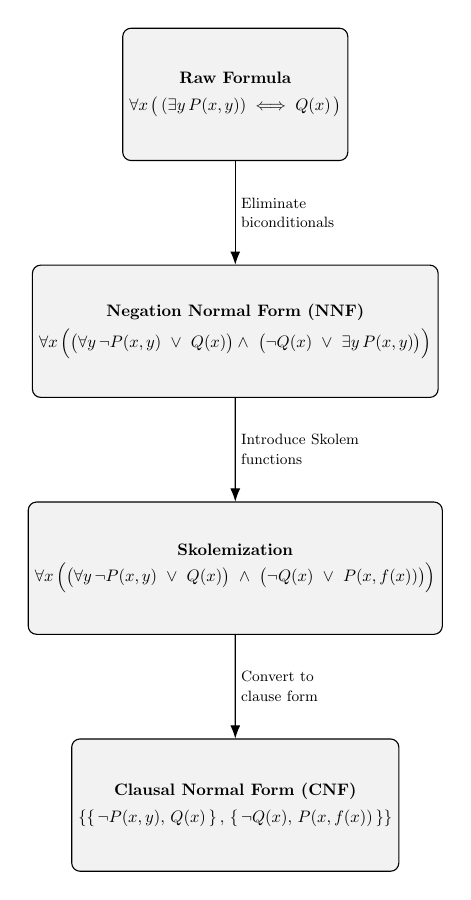
\begin{tikzpicture}[
      scale=0.6, % <-- SCALING FACTOR
      transform shape, % <-- ENSURE NODES AND TEXT ARE SCALED
      node distance=2.2cm and 0.8cm,
      stage/.style={draw, rounded corners=3pt, fill=gray!10, align=center, inner sep=4pt, minimum height=2.8cm},
      >=Latex
    ]

    % Nodes arranged vertically for better readability
    \node[stage] (raw) {\bold{Raw Formula} \\[4pt]
      \(\displaystyle \forall x \ms \big( \ms (\exists y \ms  P(x,y)) \iff Q(x) \ms \big)\)};

    \node[stage, below=of raw] (nnf) {\bold{Negation Normal Form (NNF)}\\[4pt]
      \(\displaystyle \forall x \ms \Big(\big(\forall y \ms \neg P(x,y)\ \lor\ Q(x)\big) \land\ \big(\neg Q(x)\ \lor\ \exists y \ms  P(x,y)\big)\Big)\)};


    \node[stage, below=of nnf] (sko) {\bold{Skolemization}\\[4pt]
      \(\displaystyle \forall x \ms \Big(\big(\forall y \ms \neg P(x,y)\ \lor\ Q(x)\big)\ \land\ \big(\neg Q(x)\ \lor\ P(x,f(x))\big)\Big)\)};

    \node[stage, below=of sko] (cnf) {\bold{Clausal Normal Form (CNF)}\\[4pt]
      \(\{\{ \ms \neg P(x,y), \ms  Q(x) \ms \} \ms , \ms \{ \ms \neg Q(x), \ms  P(x,f(x)) \ms \}\}\)};

    % Arrows
    \draw[->] (raw) -- node[right, text width=3cm, align=left]{\small Eliminate\\biconditionals} (nnf);
    \draw[->] (nnf) -- node[right, text width=3cm, align=left]{\small Introduce Skolem\\functions} (sko);
    \draw[->] (sko) -- node[right, text width=3cm, align=left]{\small Convert to\\clause form} (cnf);

  \end{tikzpicture}
  \caption{Clausification: Raw formula \(\rightarrow\) NNF  \(\rightarrow\) Skolemization \(\rightarrow\) CNF.}\label{fig:nnf-to-cnf-pipeline}
\end{figure}


Transforming formulae into CNF is a prerequisite for many automated reasoning techniques, particularly \emph{resolution}~\cite{chang1997}.  
By ensuring that the input is in a uniform syntactic format, inference rules can be applied in a purely mechanical way without further structural transformations.

This pipeline of transformations, combined with \emph{naming}, is also called \bold{clausification} and  constitutes the \bold{preprocessing} phase of automated reasoning systems, a crucial step to prepare formulae for \emph{inferences}.

\section{Auxiliary Predicate Introduction}\label{sec:auxiliary_predicate_introduction}

In the transformation of first-order logic (FOL) formulas, particularly when converting to clausal form, it is often advantageous to introduce \emph{auxiliary predicates} to represent complex subformulae. The general idea is to replace a subformula \(\psi(\bar{x})\) with\footnote{Here the notation \(\bar{x}\) is used as usual to indicate a sequence of variables, while the notation \(\psi(\bar{x})\) indicates a formula with \(\bar{x}\) as free variables.} a fresh predicate symbol \(P(\bar{x})\) that does not occur in the original vocabulary, and to accompany this replacement with a \emph{defining axiom} of the form
\[
\forall \bar{x}\ \big(P(\bar{x}) \iff \psi(\bar{x})\big).
\]
This method is referred to in the literature under various names, including \emph{auxiliary predicate introduction}, \emph{renaming}, and, in some contexts, \emph{axiomatization}. The defining axiom ensures that \(P\) is logically equivalent to the original subformula, thereby preserving satisfiability and logical consequence.

One of the main motivations for this technique in automated theorem proving is the avoidance of an exponential increase in formula size during \emph{clausification}.
A naïve elimination of biconditionals and the distribution of disjunctions over conjunctions can lead to a number of clauses that grows exponentially with the size of the input.
By introducing auxiliary predicates for large or deeply nested subformulae, the number of resulting clauses can be kept proportional to the size of the original formula.

Another important application arises in the context of syntactically restricted fragments of FOL, such as the \emph{guarded fragment} or the \emph{fluted fragment}.
In these fragments, unrestricted formula transformations may produce formulas that fall outside the fragment, thereby forfeiting desirable properties such as decidability or favourable complexity bounds.
Here, auxiliary predicate introduction serves as a \emph{structure-preserving} transformation: rather than expanding a subformula in a way that would violate syntactic restrictions, a fresh predicate is introduced, with a defining axiom that maintains semantic equivalence while preserving the fragment membership of the formula.

\subsection{Polarity of Subformulae}\label{subsec:polarity-of-subformulae}

The concept of \emph{polarity} provides a finer-grained analysis of where and how a subformula occurs within a larger formula.
Intuitively, polarity describes whether an occurrence of a subformula is in a \emph{positive}, \emph{negative}, or \emph{neutral} position.
A subformula occurs positively if it is under the scope of an even number of negations, and negatively if it is under the scope of an odd number of negations.
The \emph{neutral} (or \emph{zero}) polarity occurs in positions where a subformula is required in both directions of entailment, most notably when it appears under a biconditional, where neither purely positive nor purely negative reasoning suffices.

Polarity is defined inductively as follows:
\[
\begin{aligned}
&\text{(Base case)} && \mathrm{pol}(\varphi) = + \quad \text{if } \varphi \text{ is the whole formula}, \\[2pt]
&\text{(Negation)} && \mathrm{pol}(\neg \varphi) = -\mathrm{pol}(\varphi), \\[2pt]
&\text{(Conjunction / Disjunction)} && 
\begin{cases}
\mathrm{pol}(\varphi) = \mathrm{pol}(\varphi \landor \psi), \\
\mathrm{pol}(\psi) = \mathrm{pol}(\varphi \landor \psi),
\end{cases} \\[4pt]
&\text{(Implication)} && 
\begin{cases}
\mathrm{pol}(\varphi) = -\mathrm{pol}(\varphi \rightarrow \psi), \\
\mathrm{pol}(\psi) = \mathrm{pol}(\varphi \rightarrow \psi),
\end{cases} \\[4pt]
&\text{(Biconditional)} && 
\begin{cases}
\mathrm{pol}(\varphi) = 0, \\
\mathrm{pol}(\psi) = 0,
\end{cases} \quad \text{for } \varphi \leftrightarrow \psi \text{ with any polarity}, \\[4pt]
&\text{(Quantifiers)} && \mathrm{pol}(\varphi) = \mathrm{pol}(\mathcal{Q} x\, \varphi), \quad \mathcal{Q} \in \{\forall, \exists\}.
\end{aligned}
\]
Here, \(+\) denotes positive polarity, \(-\) denotes negative polarity, and \(0\) denotes neutral polarity.



\subsection{Polarity-Aware Auxiliary Predicate Introduction}\label{subsec:polarity-aware-auxiliary-predicate-introduction}

Polarity analysis allows for an optimization of auxiliary predicate introduction. If a subformula \(\psi(\bar{x})\) occurs only positively in the formula, it is sufficient to introduce the fresh predicate \(P(\bar{x})\) together with the implication
\[
\forall \bar{x}\ \big(P(\bar{x}) \implies \psi(\bar{x})\big),
\]
rather than the full biconditional. Conversely, if \(\psi(\bar{x})\) occurs only negatively, it suffices to add
\[
\forall \bar{x}\ \big(\psi(\bar{x}) \implies P(\bar{x})\big).
\]
The full biconditional is necessary only when \(\psi(\bar{x})\) occurs with zero polarity.

This optimization is widely used in \emph{definitional CNF transformations} for first-order theorem proving. By introducing only the necessary direction of the equivalence, the number of clauses generated during clausification can be reduced, often substantially, while still preserving the correctness of the transformation with respect to satisfiability and logical consequence.









    \chapter{Inference systems}\label{chap:inference-systems}

In chapter~\ref{chap:first-order-logic} we introduced FOL as a formal representation of knowledge, and we discussed its syntax and semantics.
Representation of knowledge alone is not sufficient for formalizing reasoning processes.
What is needed is a formalization of some reasoning mechanisms that can operate on this knowledge, rules that, given a set of premises, can derive new conclusions.
These rules are called \bold{inference rules}.
There are various types of inference rules, each with its own characteristics and applications.
In general, we denote with \(R\) a set of inference rules called \bold{inference system}. Given a set of premises \(\Gamma\), an inference rule \(r \in R\) can be applied to \(\Gamma\) to infer a new conclusion \(\phi\), denoted as \(\Gamma \vdash_r \phi\)\footnote{
  The notation can be simplified with just \(\Gamma \vdash \phi\) if the specific rule \(r\) is unambiguous.}.
If a sentence \(\phi\) can be inferred from the empty set using \(r\), we write \(\vdash_r \phi\).
It is possible to generalize this notation to the entire inference system \(R\) by writing \(\Gamma \vdash_{R} \phi\).
Moreover, it is possible to characterize the effectiveness of inference systems with various properties:

\begin{itemize}
    \item \bold{Soundness}: An inference system is sound if it only derives conclusions that are true in the model. Formally, \(R\) is \bold{sound} if for all \(\Gamma\) and \(\phi\), if \(\Gamma \vdash_{R} \phi\), then \(\Gamma\models\phi\).
    \item \bold{Completeness}: An inference system is complete if it can derive all conclusions that are true in the model. Formally, \(R\) is \bold{complete} if for all \(\Gamma\) and \(\phi\), if \(\Gamma\models\phi\), then \(\Gamma \vdash_{R} \phi\).
    \item \bold{Correctness}: An inference system is correct if it is both \bold{sound} and \bold{complete}.
    \item \bold{Consistency}: An inference system is consistent if it does not derive contradictory conclusions from any set of premises. Formally, \(R\) is \bold{consistent} if for all \(\Gamma\) and \(\phi\), it is not the case that both \(\Gamma \vdash_{R} \phi\) and \(\Gamma \vdash_{R} \neg \phi\).
\end{itemize}
A weaker form of completeness is \bold{refutational completeness} which requires that if \(\Gamma \models \bot\), then \(\Gamma \vdash_{R} \bot\).  Practically, this means that if a set of premises is unsatisfiable, the inference system can derive a contradiction.
By theorem~\ref{thm:validity_satisfiability_reduction}, a refutational complete inference system can show that a formula is valid by proving that its negation is unsatisfiable.
A first example of an inference rule is \bold{Modus Ponens}, which states that if we have a conditional statement \(A \implies B\), and we know that \(A\) is true, then we can conclude that \(B\) is also true. Formally, it can be expressed as:
\begin{equation}  
  \infer{B}{A & A \implies B}
\end{equation}
Or, alternatively, and more conveniently for formulae in CNF, we can express it as:
\begin{equation}  
  \infer{B}{A & \neg A \lor B}
\end{equation}
A classical application of Modus Ponens can be found in Aristotelian syllogisms, where we have two premises and a conclusion.
An example of a syllogism is:
\begin{quote}
  \emph{All humans are mortal. Socrates is a human. Therefore, Socrates is mortal}.
\end{quote}
The premises can be formalized as:
\begin{equation}
  \forall x \ms H(x) \implies M(x), \qquad H(s)
\end{equation}
These can be converted into CNF as:
\begin{equation}
    \neg H(x) \lor M(x), \qquad H(s)
\end{equation}
In FOL, before applying Modus Ponens, we must ensure that the premises contain a matching literal. To do this, we need to find the MGU \(\sigma\) that makes the literals match that, in this case, is \(\sigma = \{x\mapsto s\}\).
Finally, we can apply Modus Ponens for deriving the conclusion \(M(s)\) (Socrates is mortal) as follows:
\begin{equation}
  \infer{M(s)}{H(s) & \neg H(x) \lor M(x)}
\end{equation}

From this xample, we can define a more specific form of Modus Ponens for FOL, which takes into account the need for matching literals and the use of MGUs.
\begin{equation}  
  \infer{B\sigma}{A_1 & A_2 \implies B} \qquad \text{or} \qquad \infer{B\sigma}{A_1 & \neg A_2 \lor B}
\end{equation}
where \(\sigma\) is the MGU of \(A_1\) and \(A_2\).

While being a powerful inference rule, Modus Ponens has its limitations in the context of FOL\@.
In particular:
\begin{itemize}
  \item It is \bold{sound} because any conclusion derived is logically entailed.
  \item It is \bold{not complete} because there are valid conclusions that cannot be derived using this rule alone.
  \item It is \bold{not refutationally complete} because there are unsatisfiable sets of clauses that cannot be shown to be unsatisfiable using this rule alone.
\end{itemize}
For example, the set of clauses
\begin{equation}\label{eq:example_unsat}  
  \{\{\neg A, B\},\{\neg A , \neg B\}, \{\neg C , A\}, \{A , C\}\}
\end{equation}
This set is unsatisfiable:
\begin{description}
  \item[Assuming \(A\) true] From clause 1 we have \(B\) true, and from clause 2 we have \(\neg B\) true, leading to a contradiction.
  \item[Assuming \(A\) false] From clause 3 we have \(\neg C\) true, and from clause 4 we have \(C\) true, leading to a contradiction.
\end{description}
However, Modus Ponens alone cannot derive this contradiction because there are no atomic clauses to trigger the inference.
This limitation of Modus Ponens motivates the need for more general inference rules that can handle cases where no unit clauses are available to trigger inferences.
The resolution rule addresses this limitation by allowing inferences between any clauses containing complementary literals, regardless of their structure.

\section{Resolution and Factoring}\label{sec:resolution-factoring}

A common inference system used in FOL is based on the \bold{resolution} rule, which allows for the derivation of new clauses from existing ones, with the addition of the \bold{factoring} rule, that allows for the simplification of clauses by removing redundant literals.
The key insight is that Modus Ponens requires one premise to be a unit clause (single literal) to match against a conditional.
Resolution generalizes this by allowing any two clauses containing literals that become complementary after unification to be combined, making it much more powerful for systematic proof search in clause form.

\subsection{Resolution}\label{subsec:resolution}

\bold{Resolution} is a rule of inference specifically designed for CNF\@. It allows for the derivation of new clauses by resolving two clauses that contain complementary literals.

Formally, resolution in FOL can be defined as:

\begin{equation}
  \infer{(B\lor C)\sigma}{A_1 \lor B & \neg A_2 \lor C}
\end{equation}
\indent where \(\sigma\) is the MGU of \(A_1\) and \(A_2\).

\noindent Intuitively, resolution is justifiable noticing that, for \(A_1 \lor B\) and \(A_2 \lor C\) to be true, at least one of \(A_1\) and \(B\) must be true, and at least one of \(A_2\) and \(C\) must be true.
Being \(A_1\) and \(A_2\) complementary, it is impossible for both to be true at the same time, so at least one of \(B\) and \(C\) must be true. Thus, we can conclude that \(B \lor C\) must be true.

From this consideration, we can see that resolution is \bold{sound} because it only derives conclusions that are logically entailed by the premises.
However, resolution is \bold{not complete} because there are valid conclusions that cannot be derived using this rule alone.
An example of this is the \emph{disjunction introduction} rule \(A \models A \lor B\), which allows for the introduction of a disjunction from a single clause.
The absence of complementary literals in the premises prevents resolution from deriving any conclusions, and therefore to be complete.

Resolution though is \bold{refutationally complete}, meaning that if a set of clauses is unsatisfiable, resolution can derive the empty clause~\cite{robinson1965}, denoted \(\varnothing\), representing a contradiction --- a clause with no literals that can never be satisfied.
Using resolution, we can easily show that the previous example set of clauses~\ref{eq:example_unsat} is unsatisfiable:
\begin{equation}
  \begin{aligned}
    \neg A \lor B &\quad \text{Clause 1 (Premise)} \\
    \neg A \lor \neg B &\quad \text{Clause 2 (Premise)} \\
    \neg C \lor A &\quad \text{Clause 3 (Premise)} \\
    A \lor C &\quad \text{Clause 4 (Premise)} \\
    \neg A &\quad \text{Clause 5 (Resolution 1,2)} \\
    A &\quad \text{Clause 6 (Resolution 3,4)} \\
    \varnothing &\quad \text{Clause 7 (Resolution 5,6)}
  \end{aligned}
\end{equation}

This can be achieved by \bold{saturating} the set of clauses. A set of clauses \(S\) is \bold{saturated} under an inference system \(R\) if all the conclusions that can be derived from premises in \(S\) using inferences in \(R\) are also included in \(S\) (up to redundancy).
If the saturation of a set of clause \(S\) does contain \(\varnothing\), then \(S\) is unsatisfiable.

\subsection{Factoring}\label{subsec:factoring}

In addition to resolution, \bold{factoring} is a rule that allows for the simplification of clauses by removing redundant literals.
In contrast to the inference rules seen so far, factoring does not derive new conclusions but rather simplifies existing clauses, improving their efficiency in the proof search.

Formally, factoring can be defined as:
\begin{equation}
  \infer{(C \lor A_1)\sigma}{C \lor A_1 \lor A_2}
\end{equation}
\indent where \(\sigma\) is the MGU of \(A_1\) and \(A_2\).

\noindent Factoring eliminates duplicate literals that arise after unification. If a clause contains two literals that can be unified with MGU \(\sigma\), then applying \(\sigma\) would make them identical, and we can simplify using the tautology \(A \lor A \iff A\).

For example, from the clause \(P(x) \lor Q(y) \lor P(f(y))\), we can factor on \(P(x)\) and \(P(f(y))\) with MGU \(\sigma = \{x \mapsto f(y)\}\) to get \((P(x) \lor Q(y))\sigma = P(f(y)) \lor Q(y)\).

While resolution alone is refutationally complete, factoring serves as an optimization that reduces clause size and prevents the search space from being cluttered with subsumed clauses. This can significantly improve the performance of resolution-based theorem provers.

\section{Ordered Inferences}\label{sec:ordered-inferences}

While resolution and factoring provide a refutationally complete inference system, unrestricted application of these rules can lead to an explosion of irrelevant clauses, severely impacting efficiency. The key insight is that many inferences are redundant or unnecessary for finding a refutation.
Ordered inference rules address this problem by imposing systematic restrictions on when resolution and factoring can be applied, dramatically reducing the search space while preserving refutational completeness allowing inferences only on \emph{eligible} literals.

\subsection{Admissible Ordering}\label{subsec:admissible-ordering}

The foundation of ordered inferences is an \bold{admissible ordering} on literals, which guides the selection of inference candidates.

An ordering \(\succ\) on literals is \bold{admissible} if it satisfies:
\begin{itemize}
    \item \bold{Well-foundedness and totality on ground literals}: for any two ground literals \(L_1\) and \(L_2\), either \(L_1 \succ L_2\), \(L_2 \succ L_1\), or \(L_1 = L_2\) (totality), and each subset of ground literals has a minimal element (well-foundedness).
    \item \bold{Atom constraints}: for any atoms \(A\) and \(B\), it satisfies \(\neg A \succ A\) and \(B \succ A\) implies \(B \succ \neg A\).
    \item \bold{Stability under substitution (Liftable)}: if \(L_1 \succ L_2\), then \(L_1\sigma \succ L_2\sigma\) for any substitution \(\sigma\)
\end{itemize}

Common examples of admissible orderings include lexicographic orderings on terms and literals, where terms are compared first by their structure (function symbols, arity) and then by their arguments recursively.

For instance, using a lexicographic ordering where \(f \succ g\) and \(a \succ b\):
\[f(a) \succ f(b) \succ g(a) \succ g(b) \succ a \succ b\]

The ordering extends to literals by considering both the predicate symbols and their arguments, considering the \emph{depth} of terms.
Generally, a selection function is used to choose the most relevant literals for inference based on the admissible ordering; most of the time it is the function inducted from the ordering, selecting the maximal literals.

\subsection{Ordered Resolution}\label{subsec:ordered-resolution}

\bold{Ordered resolution} restricts the resolution rule to apply only when certain maximality conditions are satisfied.

Formally, ordered resolution can be defined as:

\begin{equation}
  \infer{(B\lor C)\sigma}{C\lor A_1 & \neg A_2 \lor B}
\end{equation}
\indent provided (i) \(\sigma\) is the MGU of \(A_1\) and \(A_2\), (ii) \(A_1\sigma\) is strictly maximal respect to \(B\sigma\), and (iii) \(\neg A_2\) is maximal with respect to \(D\sigma\).
The intuition is that we only resolve on the \dquote{largest} literals in each clause according to our ordering. This prevents resolution on smaller literals that might lead to unnecessarily complex derived clauses.

Consider the clauses:
\[P(f(x)) \lor Q(x), \qquad \neg P(y) \lor R(y)\]
If our ordering satisfies \(P(f(x)) \succ Q(x)\) and \(P(y) \succ R(y)\), then ordered resolution can proceed on the \(P\) literals, yielding:
\[Q(x) \lor R(f(x))\]
However, if \(Q(x) \succ P(f(x))\), then ordered resolution would be blocked, as \(P(f(x))\) is not maximal in the first clause.
While maintaining refutational completeness, ordered resolution, in practice, can reduce the number of generated clauses by several orders of magnitude, making automated theorem proving feasible for larger problems.
Moreover, using ordered resolution in a saturation process, can lead to termination on inputs that standard resolution cannot handle.

\subsection{Ordered Factoring}\label{subsec:ordered-factoring}

Similar restrictions apply to factoring to maintain consistency with ordered resolution.

It is defined as:
\begin{equation}
  \infer{(C \lor A_1)\sigma}{C \lor A_1 \lor A_2}
\end{equation}
\indent provided (i) \(\sigma\) is the MGU of \(A_1\) and \(A_2\), and (ii) \(A_1\sigma\) is maximal with respect to \(C\sigma\).
For example, consider the clause:
\[P(f(x)) \lor Q(y) \lor P(x)\]
If \(P(f(x)) \succ P(x) \succ Q(y)\) and we can unify \(P(f(x))\) and \(P(x)\) with \(\sigma = \{(x , f(x))\}\), then ordered factoring produces:
\[P(f(x)) \lor Q(y)\]

The combination of ordered resolution and ordered factoring creates a highly efficient inference system that maintains the theoretical guarantees of refutational completeness while achieving practical performance suitable for real-world theorem proving applications.
The ordering strategies are particularly effective because they tend to eliminate smaller, more general literals first, leading toward the specific contradictions needed for refutation more directly than unrestricted search.




    \chapter{Fluted Fragment}\label{chap:fluted-fragment}

As previously mentioned, undecidability of FOL has led to the systematic exploration of fragments that retain desirable properties while being decidable with resolution-based systems.

The definition of these fragments is tied to syntactic restrictions on the formulae, allowing the formulation of a terminating decision procedure exploiting the structure of the fragments.

Early investigations into decidable fragments often focused on restricting quantification, limiting formulae to a specific quantifier pattern.
Some notable examples are the \emph{Bernays-Schönfinkel class} (\(\exists^*\forall^*\)), the \emph{initially extended Ackermann class} (\(\exists^*\forall\exists^*\)), and the \emph{initially extended Gödel class} (\(\exists^*\forall\forall\exists^*\)).

Another notable example is the \emph{(loosely) guarded fragment}, which restricts quantification to conditional quantifiers of the form \(\forall \bar{y} (G(\bar{x},\bar{y}) \rightarrow \phi)\) or \(\exists \bar{y} (G(\bar{x},\bar{y}) \land \phi)\), where \(G\) is a \emph{guard} formula satisfying certain restrictions.

Other form of restrictions involve the arity of predicates, such as the \emph{monadic fragment}, which only allows unary predicates, or the \emph{two-variable fragment} (\(\text{FO}^2\)), which restricts formulae to at most two variables.

By contrast, the restriction of first-order logic which ensures decidability for fluted logic is an ordering on variables and arguments.

This variable-ordering approach is significant because it does not limit formulae structure or predicate arity, but only predicate application on variables.

Another significant aspect of fluted logic is the relationship to non-classical logics, such as extended modal logics and expressive description logics, which play an increasingly important role in various areas of computer science.
Fluted logic may be viewed as a generalization of modal logic, a characteristic shared with the guarded fragments. 
However, fluted logic offers advantages over guarded fragments for modal logic embeddings because it allows negation of relation atoms, enabling it to capture enriched modal logics like Boolean modal logic~\cite{gargov1990boolean}, and expressive description logics such as \(\mathcal{ALB}\) (without converse)~\cite{hustadt2000issues}.

Additionally, in~\cite{purdy1999quine} \citeauthor{purdy1999quine} describes an application in computational linguistics of fluted logics for
modelling ordinary English.

Finally, fluted logic has the finite model property~\cite{purdy1996decidability,purdy1996fluted,purdy1999quine}, which means that every satisfiable formula has a finite model.
This property is crucial because it enables decidable satisfiability checking through systematic enumeration of finite structures.

\section{Fluted Formulae}\label{sec:fluted-formulae}

Formally, the syntactic structure of fluted formulae can be defined as follows~\cite{schmidt2000resolution}:

\begin{definition}\label{def:fluted-formulae}
  Let \(\mathcal{P}\) be a finite set of predicate symbols and let \(X_m = \{x_1, \ldots, x_m\} \subseteq \mathcal{X}\)\uninatodo{this definition is taken directly from the paper but seems to not include the \(\emptyset\). Should I change it?} be an \emph{ordered} set of variables.
  An \emph{atomic fluted formula} of \(\mathcal{P} \text{ over } X_i\) is an \(n\)-ary atom \(P(x_l,\ldots, x_i)\), with \(l = i - n + 1 \text{ and } n \leq i\).
  \emph{Fluted formulae} are defined inductively as follows:
  \begin{enumerate}
    \item Any atomic fluted formula over \(X_i\) is a fluted formula over \(X_i\).
    \item \(\exists x_{i+1}\phi \text{ and } \forall x_{i+1}\phi\) are fluted formulae over \(X_{i}\), if \(\phi\) is a fluted formula over \(X_{i+1}\).
    \item Any Boolean combination of fluted formulae over \(X_i\) is a fluted formula over \(X_i\). That is, \(\phi \implies \psi, \neg \phi, \phi \land \psi\) are all fluted formulae over \(X_i\), if both \(\phi\) and \(\psi\) are.
  \end{enumerate}
\end{definition}

By definition, for any formula \(\phi\), if there is a variable renaming \(h\) such that \(h(\phi)\) is a fluted formula according to the above definition then \(\phi\) is a fluted formula.

Moreover, as a consequence of the definition, any fluted formula over \(X_i\) has \(X_i\) as its set of free variables, and therefore fluted sentences can be seen as over \(X_0 = \emptyset\).

In this definition, to quantify a fluted formula the quantified variable is forced to be the last free variable occurring in all predicate. In this sense, quantifying a formula to a sentence can be informally thought of as popping off variables from the list of free variables, which converges to \(X_0\).

% The semantics of fluted logic is defined as in FOL (\ref{subsec:semantics}).

Examples of fluted formulae are:
\begin{equation}\label{eq:fluted-example}
  \begin{aligned}
    \forall x_1 (P(x_1) \iff &\exists x_2(Q(x_2) \land R(x_1, x_2)))\\
    \forall x_1,x_2 (P(x_1,x_2) \iff &  (Q(x_1,x_2) \land\\
                                     &  \forall x_3 (R(x_1,x_2,x_3) \implies \exists x_4 Q(x_3,x_4))))
  \end{aligned}
\end{equation}

While the following examples are not fluted formulae:

\begin{equation}\label{eq:not-fluted-example}
  \begin{aligned}
    \forall x_1,x_2(P(x_1,x_2) \land \forall x_3(Q(x_3,x_1,x_2) \implies R(x_3)))\\
    \forall x_1,x_2(P(x_1,x_2) \land \exists x_3(Q(x_1,x_2,x_3) \implies \exists x_4 R(x_4,x_3)))
  \end{aligned}
\end{equation}
because the ordering of arguments is violated.

These constraints can be expressed less formally with a top-down approach as well, where the variables of atoms from a string \(fs\), where \(f\) is a possibly empty string of free variables, and \(s\) is a suffix of the string of the bound variables from the outermost quantifier to the innermost.

\begin{figure}[H]
    \centering
    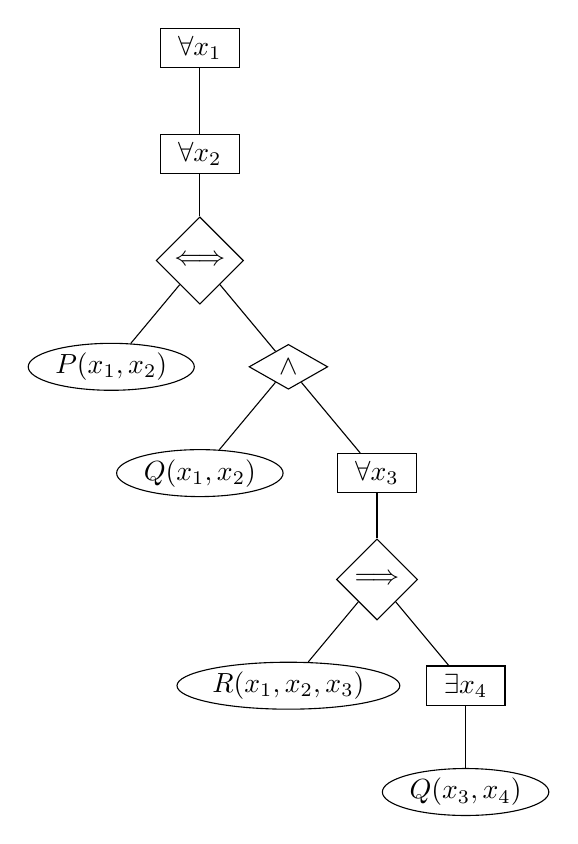
\begin{tikzpicture}[syntree, scale=0.9]
        \node[quantifier] {\(\forall x_1\)}
          child{ node [quantifier] {\(\forall x_2\)}
            child { node[connective] {\(\iff\)}
              child { node[literal] {\(P(x_1, x_2)\)} }
              child { node[connective] {\(\land\)}
                child { node[literal] {\(Q(x_1, x_2)\)} }
                child { node[quantifier] {\(\forall x_3\)}
                  child { node[connective] {\(\implies\)}
                    child { node[literal] {\(R(x_1, x_2, x_3)\)} }
                    child { node[quantifier] {\(\exists x_4\)}
                      child { node[literal] {\(Q(x_3, x_4)\)} }
                    }
                }
              }
              }
            }
          };
    \end{tikzpicture}
    \caption{Syntactic tree for last example in Equation~\ref{eq:fluted-example} without quantifiers flattening}\label{fig:fluted_syntree}
\end{figure}

\begin{figure}[H]
    \centering
    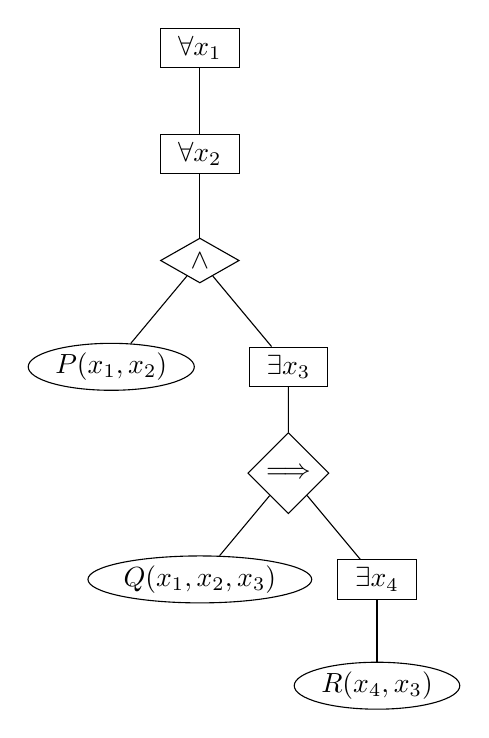
\begin{tikzpicture}[syntree,scale=0.9]
        \node[quantifier] {\(\forall x_1\)}
          child{ node [quantifier] {\(\forall x_2\)}
            child { node[connective] {\(\land\)}
              child { node[literal] {\(P(x_1, x_2)\)} }
              child { node[quantifier] {\(\exists x_3\)}
                child { node[connective] {\(\implies\)}
                  child { node[literal] {\(Q(x_1, x_2, x_3)\)} }
                  child { node[quantifier] {\(\exists x_4\)}
                    child { node[literal] {\(R(x_4, x_3)\)} }
                  }
                }
              }
            }
          };
    \end{tikzpicture}
    \caption{Syntactic tree for first example in Equation~\ref{eq:not-fluted-example} without quantifiers flattening}\label{fig:not_fluted_syntree}
\end{figure}

From the syntactic tree in Figure~\ref{fig:fluted_syntree}, it is easy to see that each atom has as arguments a suffix of the string of bound variables obtained from the traversal of the branch of the tree with the atom as leaf.

By contrast, in Figure~\ref{fig:not_fluted_syntree}, the atom \(R(x_4, x_3)\) had as argument string \(x_4 x_3\), which is not a suffix of the string of bound variables \(x_1 x_2 x_3 x_4\).

This observation leads to the fact that, in \dquote{\emph{constructing}} a fluted sentence top-down, one can only \emph{introduce} new variables at the end of the string and the variables an atom \(P\) is applied to is completely determined by the quantifiers it is in scope of and its arity, while everything remains arbitrary.

\section{Fluted Clauses}\label{sec:fluted-clauses}

In~\cite{schmidt2000resolution}, \citeauthor{schmidt2000resolution} introduces a restricted class of clauses named \bold{fluted clauses}.
These clauses are characterized by a specific structure that adheres to the constraints outlined in the previous sections and such that any fluted formula, after the necessary naming, can be transformed into a fluted clause.

Before we delve into the formal definition of the fluted clauses class, we need to introduce some notation.

The notation \(\flseq{i}\) will denote a finite, possibly empty, sequence \((u_i,u_{i+1}, \ldots, u_m)\) of terms. Unless specified otherwise each non-empty sequence \(\flseq{i}\) will be assumed to end with \(u_m\).

The sequences \(\flseq{1},\flseq{2},\ldots,\flseq{m}\) are therefore linearly ordered by the converse of the proper suffix relation and the sequence \(\flseq{m}\).
Therefore, the following notations will be used:
\begin{itemize}
  \item \(\flseq{i}[t]\) will denote the sequence \((u_i,u_{i+1}, \ldots, u_m,t)\).
  \item \(f\flseq{i}\) will denote the term \(f(u_i,u_{i+1}, \ldots, u_m)\).
  \item \(P\flseq{i}\) will denote the predicate \(P(u_i,u_{i+1}, \ldots, u_m)\).
  \item \(C\flseq{i}\) will denote a (possibly empty) clause of literals of the form \((\neg)P\flseq{i}\).
\end{itemize}

For \(f\flseq{i},P\flseq{i} \text{ and } C\flseq{i} \), \(\flseq{i}\) is called the \emph{argument sequence} of the corresponding term, predicate or clause.

If \(\flseq{i}\) is empty, then \(f\flseq{i}, P\flseq{i} \text{ and } C\flseq{i}\) respectively denote a constant, a propositional literal and a (possibly empty) propositional clause.

\begin{definition}\label{def:fluted-sequence}
Given \(m,n \in \mathbb{N} \text{ and } X_m = \{x_1,x_2,\ldots,x_m\}\) as previously defined, we will refer as to the sequence of terms \(\overline{u} = (u_1,u_2,\ldots,u_n)\) as a \emph{fluted sequence} over \(X_m\), if all the following conditions hold:
\begin{enumerate}[label= (\roman*)]
  \item \(n > m\);
  \item \(u_1=x_1,\ldots,u_m=x_m\);
  \item the number of variables occurring in \((u_{m+1},\ldots,u_n)\) is \(m\);
  \item for every \(k \in \{m+1,\ldots,n\}\), there is an \(i \in \{1,\ldots,k-1\}\) such that \\\(u_k = f(u_i,\ldots,u_{k-1})\) for some function symbol \(f\).
\end{enumerate}
The sequence \((x_1, \ldots, x_m)\) will be called the \emph{variable prefix} of \(\overline{u}\).
\end{definition}

This set of conditions serves the purpose of ensuring that the sequence of terms \(\overline{u}\) is constructed naturally extending the ordered set of variables \(X_m\) by introducing new functional terms whose argument sequences are suffixes of the \emph{fluted sequence} that precedes them.

Examples of fluted sequences are:
\begin{itemize}
  \item \((a)\), a fluted sequence over \(X_0=\emptyset\)
  \item \((x_1,x_2,x_3,f(x_1,x_2,x_3))\)
  \item \((x_1,x_2,x_3,f(x_2,x_3),g(x_1,x_2,x_3,f(x_2,x_3)))\)
  \item \((x_1,x_2,f(x_1,x_2),g(f(x_1,x_2)),h(x_2,f(x_1,x_2),g(f(x_1,x_2))))\)
\end{itemize}
while the following are not:
\begin{enumerate}[label= (\roman*)]
  \item \((x_1,x_2)\) over \(X_3\);\footnote{The sequence would have been fluted if it had been over \(X_2\) or \(X_1\) or \(X_0\).};
  \item \((x_1,x_2,f(x_3,x_4),x_3)\);
  \item \((x_1,x_2,x_3,f(x_3))\);
  \item \((x_1,x_2,x_3,f(x_3),g(x_1,x_2,x_3))\);
\end{enumerate}
because they violate respectively conditions (i), (iv), (iv) and (iv) of Definition~\ref{def:fluted-sequence}.

Moreover, these constraints ensure that the DAG representation of the fluted sequence has a unique total topological ordering providing another possible order on functional terms\footnote{Technically, the sequence ordering corresponds to the topological ordering in the \emph{transposed DAG}, with the one induced by the edges in the original DAG being its dual.}.
This can be easily shown by observing that, for every \(n\) only the vertex corresponding to \(u_n\) has in-degree zero, and therefore it must be the first vertex in any topological ordering of the DAG\@. Removing that vertex (and therefore that term) will again leave a DAG (and a fluted sequence) where only one vertex has in-degree zero (\(u_{n-1}\)), and so on until all vertices \(u_{m+1},\ldots, u_n\) are removed.

\begin{figure}[H]
\centering
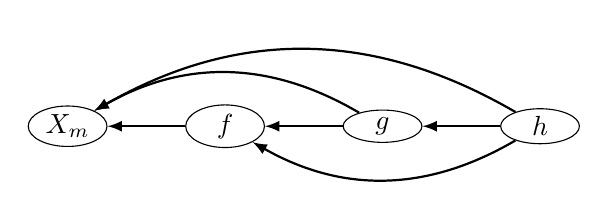
\begin{tikzpicture}[syntree]
  % Nodi
  \node[literal] (x) at (-2,0) {\(X_m\)};
  \node[literal] (f) at (0,0) {\(f\)};
  \node[literal] (g) at (2,0) {\(g\)};
  \node[literal] (h) at (4,0) {\(h\)};
  
  \draw[-latex, thick] (f) -- (x);
  \draw[-latex, thick, bend right=30] (g) to (x);
  \draw[-latex, thick] (g) -- (f);
  \draw[-latex, thick, bend right=30] (h) to (x);
  \draw[-latex, thick, bend left=30] (h) to (f);
  \draw[-latex, thick] (h) -- (g);
\end{tikzpicture}
\caption{DAG of last example of fluted sequences}
\end{figure}
Is possible now to define the class of fluted clauses.

\begin{definition}\label{def:fluted-clauses}
  A clause \(C\) is a \emph{fluted clause} over \(X_m\) if one of the following conditions holds:
  \begin{description}
    \item[(FL0)] \(C\) is a (possibly empty) propositional clause.
    \item[(FL1)] \(C\) is not empty, the set of variables occurring in \(C\) (denoted \(\var{C}\)) is exactly \(X_m\), and for any literal \(L\) in \(C\), there is some \(i \in \{1,\ldots,m\}\) such that the argument sequence of \(L\) is
      \[(x_i, x_{i+1}, \ldots, x_m).\]
    \item[(FL2)] \(C\) is functional and not empty, \(\var{C} = X_m\), and for any literal \(L\) in \(C\), the argument sequence of \(L\) is one of
      \[(x_{i},x_{i+1}, \ldots, x_{i_m}) \text{ or }\]
      \[(u_j, u_{j+1}, \ldots, u_{n}),\]
    where \(1 \leq i \leq m\) and \((u_j, u_{j+1}, \ldots, u_{n})\) is a suffix of some fluted sequence \(\overline{u} \text{ over } \{x_k, \ldots, x_m\}\) with \(k \in \{1,\ldots,m\}\).
    \(\overline{u}\) will be referred to as the \emph{fluted sequence associated} with \(L\).
    \item[(FL3)] \(C\) is not empty, \(\var{C} = X_{m+1}\), and for any literal \(L\) in \(C\), the argument sequence of \(L\) is either
      \[(x_{1},x_{2}, \ldots, x_{m}) \text{ or }\]
      \[(x_{i},x_{i+1}, \ldots, x_{m},x_{m+1}),\]
    where \(1 \leq i \leq m+1\).
  \end{description}
  A fluted clause will be called \emph{strongly fluted clause} if it is either ground or has a literal which contains all the variables of the clause.
\end{definition}

Some examples of fluted clauses are:
\begin{description}
  \item[(FL0)] \(\neg P \lor Q \lor R\)
  \item[(FL1)] \(P(x_1,x_2,x_3,x_4,x_5) \lor Q(x_1,x_2,x_3,x_4,x_5) \lor \neg R(x_4,x_5) \lor S(x_5)\)
  \item[(FL2)] \(Q(x_1,x_2) \lor R(x_2) \lor P(x_1,x_2,f(x_1,x_2))\lor R(x_2,f(x_1,x_2)) \lor S(f(x_1,x_2))\)
  \item[(FL3)] \(Q(x_1,x_2) \lor \neg P(x_1,x_2,x_3) \lor \neg R(x_2,x_3) \lor S(x_3)\)
\end{description}

Some additional notes:
\begin{enumerate*}[label= (\alph*)]
  \item The non-functional subclause of a (FL2)-clause (denoted by \(\nabla\)) satisfies (FL1), therefore (FL1)-clauses are building blocks of (FL2)-clauses.
  \item Clauses of type (FL3) are defined to be fluted clauses over \(m\) variables, even though they contain \(m+1\) variables. This is to ensure direct association of fluted formulae over \(m\) variables with fluted clauses over \(m\) variables. The previous example of (FL3)-clause is therefore over \(2\) variables.
  \item No fluted clause can simultaneously satisfy multiple fluted conditions at once.
\end{enumerate*}

Strongly fluted clauses will be the core of the resolution procedure assuring its termination.
That is because, resolving two strongly fluted clauses and selecting as eligible literal the literal containing all the variable of the clause, will produce a resolvent with a number of variables less than or equal to the number of variables of the parent clauses.

Some additional property of fluted clauses come from the following results.
The proofs follow straightforwardly and are therefore omitted for brevity. Complete demonstration for these lemmas, and for all other claims in this chapter, can be found in~\cite{hustadt2000resolution}.

\begin{lemma}\label{lem:fluted-sequence-properties}
  Let \(\overline{u}\) be a fluted sequence over \(X_m\). Then:
  \begin{enumerate}
    \item There is an element \(u_k\) of \(\overline{u}\) such that \(u_k = f(u_1,\ldots,u_{k-1})\), for some \(f\)
    \item If \(u_n\) is the last element of \(\overline{u}\), then \(\var{u_n} = X_m\)
    \item \(\overline{u}\) is uniquely determined by its last element
    \item if \(u_j, u_{j+1}, \ldots, u_n\) is a suffix of \(\overline{u}\), then \(u_1, \ldots, u_{j-1}\) is uniquely determined by \(u_j\)
  \end{enumerate}
\end{lemma}

\begin{lemma}\label{lem:var-sequence-fl2}
  Let \(L\) be any literal of a (FL2)-clause defined over \(X_m\). Then, all occurrences of variable sequences in \(L\) are suffixes of \(x_1, \ldots, x_m\).
\end{lemma}

\begin{lemma}\label{lem:strongly-fluted-clauses}
  Let \(C\) be a fluted clause over \(m\) variables. \(C\) is strongly fluted if and only if:
  \begin{enumerate*}[label= (\roman*)]
    \item \(C\) satisfies exactly one of the conditions (FL0), (FL1), (FL2), or
    \item \(C\) satisfies condition (FL3), and it contains a literal with \(m+1\) variables.
  \end{enumerate*}
\end{lemma}

Lemma~\ref{lem:strongly-fluted-clauses} is of particular relevance, because it assures that any fluted clause is indeed strongly fluted, except for some (FL3)-clauses. Those exceptions will be handled with a new inference rule named \emph{separation} that will be introduced later.

\section{From Fluted Formulae to Fluted Clauses}\label{sec:from-fluted-formulae-to-fluted-clauses}

Once defined the class of fluted clauses, a procedure to transform any fluted formula into a set of fluted clauses is needed.

This transformation is obtained by pre-pending to standard clausification defined in Section~\ref{sec:skolemization_and_normalization} a step of \emph{renaming}, as mentioned in Section~\ref{sec:auxiliary_predicate_introduction}, that guarantees the preservation of the fluted structure.

In particular, the renaming technique used is also known as \emph{structural transformation}.

To describe this \emph{renaming} step more formally it is sufficient to define a function that maps any fluted formula \(\phi\) over \(X_m\) to a fluted formula \(t(\phi)\) over \(X_m\) that, after the standard clausification, produces a set of fluted clauses.

Let \(Pos(\phi)\) be the set of positions of a first-order formula \(\phi\). If \(\lambda\) is in \(Pos(\phi)\), then \(\phi|_\lambda\) denotes the subformula of \(\phi\) at position \(\lambda\) and, extending the previously introduced notation for substitution, \(\phi[\psi\mapsto\lambda]\) is the result of replacing \(\phi|_\lambda\)  at position \(\lambda\) with \(\psi\).

Looking at formulae from the prospective of their syntactic tree, \(Pos(\phi)\) can be seen as the set of all nodes in the tree visited in a pre-order traversal, \(\phi|_\lambda\) is the subtree rooted at node \(\lambda\), and \(\phi[\psi\mapsto\lambda]\) is tree obtained by replacing the subtree rooted at node \(\lambda\) with the tree of \(\psi\).
Structural transformations associates with each element \(\lambda \in \Lambda \subseteq Pos(\phi)\) a fresh predicate symbol \(Q_\lambda\) and a literal \(Q_\lambda(x_1,\ldots,x_n)\), where \(x_1,\ldots,x_n\) are the free variables of \(\phi|_\lambda\), such that any two symbols \(Q_\lambda \text{ and } Q_{\lambda'}\) are equal only if \(\phi|_\lambda\) and \(\phi|_{\lambda'}\) are equivalent formulae.

Let 
  \[\fldef{\lambda}[+]{\phi} = \forall x_1, \ldots, x_n(Q_\lambda(x_1,\ldots,x_n)\implies \phi|_\lambda) \text{ and}\]
  \[\fldef{\lambda}[-]{\phi} = \forall x_1, \ldots, x_n(\phi|_\lambda \implies Q_\lambda(x_1,\ldots,x_n)).\]

The \emph{definition} of \(Q_\lambda\) is the formula
\begin{equation}
  \fldef{\lambda}{\phi} = \begin{cases}
                        \fldef{\lambda}[+]{\phi} & \text{if } \phi|_\lambda \text{has positive polarity}\\
                        \fldef{\lambda}[-]{\phi} & \text{if } \phi|_\lambda \text{has negative polarity}\\
                        \fldef{\lambda}[+]{\phi} \land \fldef{\lambda}[-]{\phi} & \text{otherwise}
                      \end{cases}
\end{equation}
The corresponding clauses are called \emph{definitional clauses}.

Is possible to inductively extends \emph{definition} to the whole set of positions \(\Lambda\) (\(Def_\Lambda(\phi)\)) as follows:
\begin{equation}
  \begin{aligned}
    \fldef{\emptyset}{\phi} &= \phi\\
    \fldef{\Lambda\cup\{\lambda\}}{\phi} &= \fldef{\Lambda}{\phi[Q_\lambda(x_1,\ldots,x_n)\mapsto\lambda]} \land \fldef{\lambda}{\phi}
  \end{aligned}
\end{equation}
where \(\lambda\) is maximal in \(\Lambda\cup\{\lambda\}\) with respect to the prefix ordering on positions.

For any first-order formula \(\phi\), \(\fldef{\Lambda}{\phi}\) will denote the \emph{definitional form} obtained by introducing new names for subformulae at positions in \(\Lambda\).
This transformation can be seen as substituting each node of the syntactic tree in \(\Lambda\) with a fresh literal \(Q_\lambda(x_1,\ldots,x_n)\) in post-order, adding the definition of \(Q_\lambda\) as a child of a new root node for the \(\land\) connective.

\begin{figure}[H]
  \centering
  \begin{minipage}[t]{.3\textwidth}
    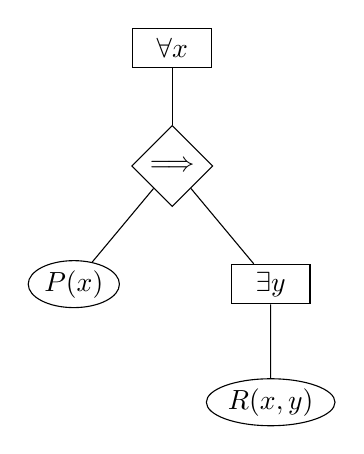
\begin{tikzpicture}[syntree]
      \node[quantifier] {\(\forall x\)}
            child { node[connective] {\(\implies\)}
              child { node[literal] {\(P(x)\)} }
              child { node[quantifier] {\(\exists y\)}
                  child { node[literal] {\(R(x, y)\)} }
              }
            };
    \end{tikzpicture}
  \end{minipage}
  \begin{minipage}[t]{.3\textwidth}
    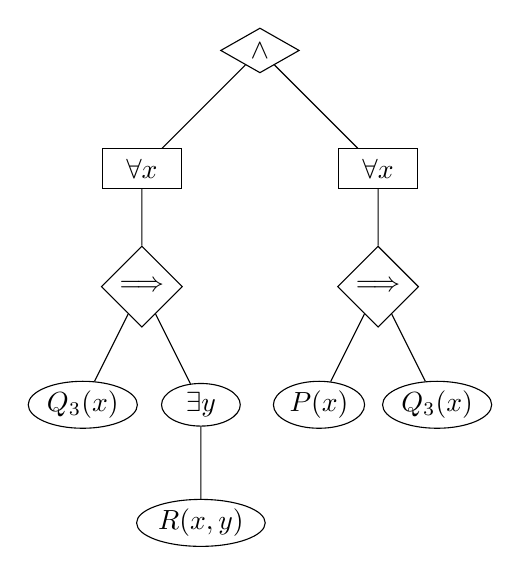
\begin{tikzpicture}[syntree,
                        level 1/.style={sibling distance=3cm},
                        level 2/.style={sibling distance=2cm},
                        level 3/.style={sibling distance=1.5cm}
                        ]
      \node[connective] {\(\land\)}
            child {node[quantifier] {\(\forall x\)}
              child { node[connective] {\(\implies\)}
                child { node[literal] {\(Q_3(x)\)} }
                child { node[literal] {\(\exists y\)}
                  child { node[literal] {\(R(x, y)\)} }
                }
              }
            }
            child{node[quantifier] {\(\forall x\)}
              child { node[connective] {\(\implies\)}
                child { node[literal] {\(P(x)\)} }
                child { node[literal] {\(Q_3(x)\)} }
              }
            };
    \end{tikzpicture}
  \end{minipage}
  \caption{Structural transformation of a formula into its definitional form with \(\Lambda = \{3\}\).}\label{fig:definitional-form}
\end{figure}

Usually \(\Lambda\) is the subset of all positions of subformulae which are non-atomic or non-literal.

For the problem of decidability is important that this transformation preserves satisfiability. Indeed, the following theorem holds:

\begin{theorem}\label{thm:definitional-sat-preservation}
  Let \(\phi\) be a first-order formula. For any \(\Lambda \subseteq Pos(\phi)\),
  \begin{enumerate}
    \item \(\phi\) is satisfiable if and only if \(\fldef{\Lambda}{\phi}\) is satisfiable;
    \item \(\fldef{\Lambda}{\phi}\) can be computed in polynomial time.
  \end{enumerate}
\end{theorem} 

It is therefore possible to show that any fluted formula \(\phi\), introducing new literals for each non-literal subformula position, can be transformed into a set of strongly fluted clauses.

\begin{lemma}
  Let \(\phi\) be any fluted formula. If \(\Lambda\) contains all non-literal subformulae positions of \(\phi\) then the clausification of \(\fldef{\Lambda}{\phi}\) is a set of strongly fluted clauses (provided the newly introduced literals have the form \((\neg)Q_\lambda(\overline{x}_i)\)).
\end{lemma}

To instead obtain a set of fluted clauses (not necessarily strongly fluted) it is required to introduce new symbols only for the quantified subformulae\footnote{Technically in~\cite{hustadt2000resolution} is mentioned, that only requires the introduction of new symbols for positive occurrences of universally quantified subformulae, negative occurrences of existentially quantified subformulae and all quantified subformulae with zero polarity, but then another form of Skolemization needs to be used. }.

\begin{lemma}\label{lem:fluted-def-constraints}
  Let \(\phi\) be any fluted formula over \(X_m\). If \(\Lambda\) contains at least the positions of any subformulae \(\exists x_{i+1}\psi, \forall x_{i+1}\psi\), then the clausification of \(\fldef{\Lambda}{\phi}\) is a set of fluted clauses (again, provided the newly introduced literals have the form \((\neg)Q_\lambda(\overline{x}_i)\)).
\end{lemma}

The loss of strong property of the generated clauses is due to \(\fldef{\lambda}[-]{\phi}\) of existentially quantified subformulae (and to \(\fldef{\lambda}[+]{\phi}\) of universally quantified subformulae by duality).
This is easy to show considering the subformula at position \(\lambda\):
  \[
    \exists x_3 (P(x_1,x_2,x_3) \lor R(x_2,x_3))
  \]
that leads to the negative definition
  \[
    \fldef{\lambda}[-]{\phi} = \forall x_1,x_2(\exists x_3 (P(x_1,x_2,x_3) \lor R(x_2,x_3)) \implies Q_\lambda(x_1,x_2))
  \]
whose clausification to the (FL3)-clauses
  \[
    Q_\lambda(x_1,x_2) \lor \neg P(x_1,x_2,x_3)
  \]
  \[
    Q_\lambda(x_1,x_2) \lor \neg R(x_2,x_3)
  \]
of which the latter does not contain a literal which contains all the variables of the clause, and is thus only fluted, not strongly fluted.

Having only fluted clauses and not strongly fluted ones in this phase is not a problem because, as we will see later, resolution of strongly fluted clauses can produce a non-strongly fluted clauses, making a procedure to obtain equivalent strongly fluted clauses from non-strongly fluted ones necessary anyway.

This procedure is the new inference rule named \bold{separation}.
\section{Separation}\label{sec:separation}
As briefly mentioned in the previous section, the motivation for introducing the \emph{separation} inference rule is that the class of fluted clauses is not closed under resolution.
In particular, resolvents of non-strongly fluted (FL3)-clauses are not always fluted and can cause (potentially) unbound variable chaining across literals.

This can be shown considering the resolution between
  \[
    P_1(x_1,x_2) \lor Q_1(x_2,x_3) \lor R(x_2,x_3) \text{ and }
  \]
  \[
  \neg R(x_1,x_2) \lor P_2(x_1,x_2) \lor Q_2(x_2,x_3)
  \]
which produces the resolvent
  \[
    P_1(x_1,x_2) \lor Q_1(x_2,x_3) \lor P_2(x_2,x_3) \lor Q_2(x_3,x_4)
  \]
that is not fluted and contains more variables than the original clauses.

The class of strongly fluted clauses is also not closed under resolution but, inferences with two strongly fluted clauses always produce fluted clauses, and non-strongly fluted clauses are what we call separable and can be restored to strongly fluted clauses.

Consider the strongly fluted clauses
  \[
    P(x_1,x_2) \lor R(x_1,x_2,x_3) \text{ and }
  \]
  \[
  \neg R(x_1,x_2,x_3) \lor P(x_2,x_3)
  \]
whose resolvent is
  \[
    C = P(x_1,x_2) \lor P(x_2,x_3)
  \]

\(C\) satisfies (FL3) but it is not strongly fluted, as none of its literals contains all the variables of the clause.

A consequence of this, is that the literals are incomparable under an admissible ordering (in particular, a liftable ordering), because the literals have a common instance, for example
  \[
    C\{x_1 \mapsto a, x_2 \mapsto a, x_3 \mapsto a\} = P(a,a) \lor P(a,a)
  \]

The problem is caused by the variable \(x_1 \text{ and } x_3\). Because they do not occur together in any literal, \(C\) can be separated and replaced by the following two clauses, where \(Q\) is a new predicate symbol.
  \[
    Q(x_2) \lor P(x_1,x_2)
  \]
  \[
    \neg Q(x_2) \lor P(x_2,x_3)
  \]
These two clauses are indeed strongly fluted, the first satisfying (FL1) and the second (FL3) but being strongly fluted.

This process of separating non-strongly fluted clauses into strongly fluted can be formalized in the \bold{separation} inference rule, that can be used outside the context of fluted logic as well.

\begin{definition}
  Let \(C\) be an arbitrary clause. \(C\) is \bold{separable} if it can be partitioned into two non-empty subclauses \(D_1\) and \(D_2\) such that \(\var{D_1} \not\subseteq \var{D_2} \text{ and } \var{D_2} \not\subseteq \var{D_1}\)
\end{definition}

For example the clause shown before is separable, while the clause
\[
P(x_1,x_2) \lor Q(x_2,x_3) \lor R(x_1,x_3)
\]
is not separable.
\begin{theorem}\label{thm:separation}
  Let \(C \lor D\) be a separable clause such that \(\var{C} \cap \var{D} = \{x_1,\ldots,x_n\}\) for \(n \in \mathbb{N}\).
  Let \(Q\) be a fresh predicate symbol with arity \(n\).
  Then a set of clauses \(N \cup \{C\lor D\}\) is satisfiable if and only if the set of clauses \(N \cup \{\neg Q(x_1,\ldots, x_n) \lor C, Q(x_1,\ldots, x_n) \lor D\}\) is satisfiable.
\end{theorem}

On the basis of this theorem we can define the following replacement rule:

\begin{equation}\label{eq:separation-rule}
  \bold{Separation:} \quad \infer{N \cup \{\neg Q(x_1,\ldots, x_n) \lor C, Q(x_1,\ldots, x_n) \lor D\}}{N \cup \{C \lor D\}}
\end{equation}
\indent provided 
\begin{enumerate*}[label = (\roman*)]
  \item \(C \lor D\) is separable,
  \item \(\var{C} \cap \var{D} = \{x_1,\ldots,x_n\}\) for \(n \in \mathbb{N}\),
  \item \(Q\) is \indent a fresh predicate symbol with arity \(n\).
\end{enumerate*}

From the definition of separable clauses, also follows that
\begin{lemma}\label{lem:separation-replacement}
  The replacements of a separable clause \(C\) each contain less variable than \(C\)
\end{lemma}

Moreover, it is possible to prove the following.

\begin{theorem}
  Let \(R^{sep}\) denote the extension of \(R\) defined as in Section~\ref{sec:resolution-factoring} with the separation inference rule and let \(N\) be a set of clauses.
  Then \(N\) is unsatisfiable if and only if the saturation of \(N\) under \(R^{sep}\) contains the empty clause.
\end{theorem}

More generally, this theorem holds also if \(R^{sep}\) is based on ordered resolution

By Lemma~\ref{lem:strongly-fluted-clauses}, separable fluted clauses have the form
\begin{equation}\label{eq:separable-fluted-clauses}
  \mathcal{L}(\overline{x}_1)\lor \mathcal{L}(\overline{x}_i,x_{m+1}) \lor \ldots \lor \mathcal{L}(x_m, x_{m+1}) \lor \mathcal{L}(x_{m+1})
\end{equation}
where \(\mathcal{L}(\cdot)\) denotes a (possibly empty) disjunction of literals with non-empty argument sequence \((\cdot)\), \(\mathcal{L}(\overline{x}_1)\) is not empty and \(i\) is the smallest integer in \(\{2,\ldots, m\}\) such that \(\mathcal{L}(\overline{x}_i), x_{m+1}\) is not empty.

The separation of clauses i this form, will produce clauses with the form
\[
  \neg Q(\overline{x}_i) \lor \mathcal{L}(\overline{x}_1) \text{ and }
\]
\[
  Q(\overline{x}_i) \lor \mathcal{L}(\overline{x}_i,x_{m+1}) \lor \ldots \lor \mathcal{L}(x_m, x_{m+1}) \lor \mathcal{L}(x_{m+1})
\]
which are obviously strongly fluted, thanks to literals in \(\mathcal{L}(\overline{x}_1)\) and in \(\mathcal{L}(\overline{x}_i)\).

From this, follows that:
\begin{lemma}\label{lem:separation-fluted}
  The separation of a separable fluted clause~\ref{eq:separable-fluted-clauses} is a set of strongly fluted clauses
\end{lemma}
\begin{lemma}
  For fluted clauses a separation inference step can be performed in linear time
\end{lemma}


\section{Fluted Resolution}\label{sec:fluted-resolution}

In the end, we can formally define an ordered resolution based inference system \(R^{sep}\) whose application is a decision procedure for fluted logic.

The ordering \(\succ\) of \(R^{sep}\) is required to be any admissible ordering compatible with the following complexity measure.

\begin{definition}
  Let \(\succ_s\) denote the proper super-term ordering. Define the complexity measure of any literal \(L\) by \(c_L = (ar(L),max(L),sign(L))\), where \(ar(L)\) is the arity of \(L\), \(max(L)\) is a \(\succ_s\)-maximal term occurring in \(L\) and \(sign(L)\) is \(1\) if \(L\) is negative and \(0\) if \(L\) is positive. % chktex 35
  The ordering on the complexity measures is given by the lexicographic combination of \(>,\succ_s \text{ and } >\), where \(>\) is the usual ordering on natural numbers.
\end{definition}

Having the ordering \(\succ\) in place, we can now define the inference system \(R^{sep}\) more formally.

\begin{definition}
  Let \(R^{sep}\) be any inference system in which
  \begin{enumerate*}[label = (\roman*)]
    \item derivations are generated by removing redundant literals, separating separable clauses and deducing new clauses with the inferences in \(R\) in this order
    \item the ordering is based on \(\succ\), defined above.
  \end{enumerate*}
\end{definition}

It can be shown that the class of fluted clauses is closed under the inference system \(R^{sep}\) by the following lemmas.

\begin{lemma}\label{lem:factor-strongly-fluted}
  A factor of a strongly fluted clause \(C\) is again a strongly fluted clause of the same type.
\end{lemma}
In fact, any (unordered) factor of a strongly fluted clause \(C\) is again a strongly fluted clause of the same type.

\begin{lemma}
  Let \(C = C' \lor A_1\) and \(D = \neg A_2 \lor D'\) be (FL2)-clauses.
  Suppose \(A_1\) and \(A_2\) are eligible literals in \(C\) and \(D\) respectively, and that \(\sigma\) is the MGU of \(A_1\) and \(A_2\).
  Then:
  \begin{enumerate}
    \item \(C\sigma\), \(D\sigma\) and \(C\sigma \lor D\sigma\) are (FL2)-clauses.
    \item For any functional literal \(L\sigma\) in \(C\sigma \lor D\sigma\), the fluted sequence associated with \(L\sigma\) is the \(\sigma\)-instance of a fluted sequence \(\overline{v}\) associated with some literal \(L'\) in \(C \lor D\).
  \end{enumerate}
\end{lemma}

This lemma is the most important technical result of~\cite{hustadt2000resolution} because with it, we can easily show that the resolution of strongly fluted clauses involving (FL2)-clauses always produce strongly fluted clauses.
\begin{lemma}\label{lem:union-strongly-fluted}
  Let \(C = C' \lor A_1\) and \(D = \neg A_2 \lor D'\) be strongly fluted clauses. Suppose \(A_1\) and \(A_2\) are eligible literals in \(C\) and \(D\) respectively, and that \(\sigma\) is the MGU of \(A_1\) and \(A_2\).
  Then \(C\sigma \lor D\sigma\) is a strongly fluted clause.
\end{lemma}
\begin{lemma}\label{lem:removal-fluted}
  Removing any subclause from a fluted clause produces a fluted clause.
\end{lemma}
The combination of Lemmas~\ref{lem:union-strongly-fluted} and~\ref{lem:removal-fluted} leads to the closure of fluted clauses under ordered resolution.

\begin{lemma}\label{lem:resolution-fluted}
  The resolvent of any two strongly fluted clauses is a strongly fluted clause, or, it is only a fluted clause, if one of the premises is a (FL3)-clause
\end{lemma}

Moreover, it can be shown that:

\begin{lemma}\label{lem:size-fluted}
  Let \(C,D\) and \(\sigma\) defined as in Lemma~\ref{lem:union-strongly-fluted}. Then,
  \[ |\var{C\sigma \lor D\sigma} \leq \max\{ |\var{C\sigma}|,|\var{D\sigma}|\}\]
\end{lemma}
Finally, by Lemmas~\ref{lem:separation-fluted},~\ref{lem:factor-strongly-fluted} and~\ref{lem:resolution-fluted}, we can conclude that:
\begin{lemma}
  Any separated factor or resolvent of strongly fluted clauses is strongly fluted.
\end{lemma}

In the end, remains only to show that the application of \(R^{sep}\) constitutes a decision procedure for fluted logic, and so does terminate on each finite input set of clauses.

For doing this it is usually sufficient~\cite{joyner1976resolution} to show that:
\begin{enumerate}[label= (\roman*)]
  \item\label{item:bounded-variables} the number of variables in any derivable clause is finitely bounded;
  \item\label{item:bounded-depth} there is a bound on the depth of terms occurring in derived clauses;
  Because separation introduces new predicate names during the derivation, in our case we also need to show that:
  \item\label{item:bounded-separation} there is a bound on the number of applications of the separation rule.
\end{enumerate}

From Lemmas~\ref{lem:separation-replacement} and~\ref{lem:size-fluted}, follows immediately~\ref{item:bounded-variables} by:
\begin{lemma}\label{lem:bounded-variables}
  All clauses occurring in an (\(R^{sep}\))-derivation from \(N\) contain at most \(m+1\) variables, where \(m\) is the maximal arity of any predicate symbol in \(N\)
\end{lemma}

The definition of fluted clauses places no restriction on the level of nesting of functional terms. But:
\begin{lemma}\label{lem:bounded-depth}
  A bound on the maximal term depth of clauses derived by \(R^{sep}\) from \(N\) is \(m\), where \(m\) is the maximal arity of any predicate symbol in \(N\)
\end{lemma}
This lemma can be shown by observing that, as a consequence of Lemma~\ref{lem:strongly-fluted-clauses}, the maximal length of any fluted sequences associated with literals in inferred clauses does not increase and that the maximal term depth of any term is the length of the fluted sequence associated with it.
It follows that the maximal term depth for any derived clause is the maximal length of any fluted sequence of a literal in \(N\) that, is obviously \(m\), the maximal arity of any predicate symbol in \(N\).

Finally, remains to show~\ref{item:bounded-separation}.

\begin{lemma}\label{lem:bounded-separation}
  The number of applications of the separation rule in any (\(R^{sep}\))-derivation from \(N\) is bounded.
\end{lemma}

The idea of the proof is that the newly introduced literals is never eligible in the new clauses because its arity is always less than some literal in the clause.
Therefore, the two replacement of a separated clause cannot be resolved together recreating the original clause. The literals become eligible only when all other \dquoteit{bigger} literals are removed, leading to a non-increase of arity.

The theoretical discussion of the fluted fragment can therefore be said to be concluded with the enunciation of the last final theorem deriving directly from the previous lemmas.

\begin{theorem}
  Let \(\phi\) be any fluted formula and \(N\) be the clausification of \(\fldef{\Lambda}{\phi}\) satisfying the restrictions of Lemma~\ref{lem:fluted-def-constraints}.
  Then:
  \begin{itemize}
    \item Any \(R^{sep}\)-derivation from \(N\) terminates.
    \item \(\phi\) is unsatisfiable if and only if the \(R^{sep}\)-saturation of \(N\) contains the empty clause.
  \end{itemize}
\end{theorem}

\begin{proof}
  Termination is a consequence of Lemmas~\ref{lem:bounded-variables},~\ref{lem:bounded-depth} and~\ref{lem:bounded-separation}, while soundness and completeness follows from~\cite{robinson1965} alongside Theorems~\ref{thm:definitional-sat-preservation} and~\ref{thm:separation}, in conjunction with Lemma~\ref{lem:bounded-separation}
\end{proof}





    \chapter{Vampire Theorem Prover}\label{chap:vampire-theorem-prover}
Having established the theoretical foundations of first-order logic, resolution-based inference systems, and the fluted fragment in the preceding chapters, we now turn to the practical implementation aspects of our decision procedure.
The implementation described in this thesis is built as an extension to Vampire~\cite{kovacs2013vampire,AVATAR,riazanov2002design}, a state-of-the-art first-order theorem prover written in C++ that employs a sophisticated array of techniques to automate reasoning tasks, including resolution-based methods, superposition calculus, and various preprocessing strategies.
It is widely used in both academic research and industrial applications for its efficiency and effectiveness in solving complex logical problems across diverse domains.
Its open-source nature and carefully designed modular architecture allow for easy integration of new techniques and algorithms, making it a flexible and extensible platform for researchers and practitioners in automated reasoning.

The system's development began in 1998 as a research project by \citeauthor{riazanov2002design} at the University of Manchester, and it is currently maintained by a broader team in the Computer Science department.
Over more than two decades of active development, Vampire has evolved into one of the most sophisticated theorem provers available, incorporating numerous theoretical advances from the automated reasoning community and practical optimizations derived from extensive empirical evaluation.
This long development history has resulted in a mature system that balances theoretical soundness with practical performance considerations.

Vampire's most defining quality is its exceptional efficiency, which has been the primary focus of its development and a key factor in establishing its prominence within the automated theorem proving community.
This efficiency is consistently demonstrated through its outstanding performance in the annual CADE ATP System Competition (CASC), the premier international competition for automated theorem provers.
Vampire has maintained a position among the top-performing systems for many years, winning in at least one category annually and achieving a particularly impressive milestone in 2025 when Vampire 5.0 secured victories in all competition categories.
These consistent competitive successes reflect not only the system's computational efficiency but also the effectiveness of its proof search strategies and heuristic selection mechanisms.

However, this relentless focus on efficiency has resulted in significant trade-offs regarding code readability and maintainability.
While the high-level architecture and component design are well-documented in various academic papers, the actual implementation is often complex and lacks comprehensive documentation.
This complexity makes it challenging for new contributors to understand and work with the codebase, frequently requiring them to \dquoteit{reverse engineer} existing functionality to understand the intricate details of specific algorithms and their implementations.
The situation is further complicated by recent development efforts that, while attempting to improve code organization, have removed, replaced, or restructured several components, making extensions written for previous versions incompatible with newer releases.
This creates additional challenges for researchers who have invested effort in developing custom modifications to the system.

This chapter provides a high-level overview of the Vampire components that are essential for understanding our implementation.
We focus particularly on the preprocessing pipeline (Section~\ref{sec:preprocessor}), the saturation algorithm (Section~\ref{sec:saturation-algorithm}) with its literal selection mechanisms (Section~\ref{subsec:literal-selection}), and the AVATAR architecture (Section~\ref{sec:avatar-architecture}), which we had to disable during our experimental evaluation.
While Vampire encompasses many additional sophisticated features, we limit our discussion to those aspects that directly influence or interact with our fluted fragment decision procedure.
It should be noted that both this description and the development work are based on Vampire version 4.9, which is the latest version available at the time of writing.

\section{Components Overview}\label{sec:components-overview}

\begin{figure}[H]
  \centering
  \includegraphics[width=0.8\textwidth]{4-vampire-theorem-prover/Vampire-package-diagram.pdf}
  \caption{Vampire theorem prover modular architecture overview.}\label{fig:vampire-architecture}
\end{figure}

Vampire's architecture is organized around a modular design that divides computational responsibilities across distinct modules, each handling specific aspects of the theorem proving process.
\uninatodo{Update UMLs with correct names in classes}

The \code{Kernel} module serves as the central component containing the system's fundamental data structures and control mechanisms.
This module houses representations for \bold{terms}, \bold{clauses}, and \bold{formulae}, which form the basic building blocks of first-order logic manipulation within Vampire.
The Kernel also contains the \code{Main Loop} of the program, which coordinates the overall execution flow and manages interactions between the various modules.

Several modules address specific computational tasks within the theorem proving process.
The \code{Parse} module handles the parsing of input problems expressed in various standard formats.
The \code{Saturation} module implements the saturation algorithms that drive the theorem proving process, systematically exploring logical consequences through controlled inference generation and clause management.
The \code{Inferences} module provides implementations of the inference rules employed during saturation, encapsulating the logical transformations that generate new clauses from existing ones.

The system includes several utility modules that provide supporting functionality.
The \code{Lib} module contains fundamental data structures used throughout the system, along with utility functions for manipulating these structures.
These components are designed to handle the specific access patterns and performance requirements typical of theorem proving applications.

The \code{Indexing} module provides data structures and algorithms for efficient storage, retrieval, and matching of terms during the reasoning process.
This module enables unification operations and term matching, which are required for the application of inference rules.
The performance characteristics of these indexing mechanisms directly affect the overall speed of the theorem prover.

User interaction and system configuration are managed by the \code{Shell} module, which handles command-line argument processing, configuration file management, and the various options that control Vampire's behaviour during execution.
This module translates user specifications and problem files into the internal representations required by the core modules.
It also contains preprocessing functionality to prepare the input for the theorem proving process.

Finally, the \code{Debug} module provides infrastructure for performance analysis and system monitoring.
It contains classes and macros for time measurements, statistics collection, and debugging support that enable performance analysis and system optimization.



\section{Problems Representation}\label{sec:problems-representation}

Vampire represents logical problems using a combination of data structures that encapsulate the various components of first-order logic.

\subsection{Terms and Literals}\label{subsec:terms-and-literals}

As discussed earlier, terms and literals are the basic building blocks of first-order logic expressions, and they therefore need to be represented in the most efficient way possible.

In Vampire, terms are represented by the \code{TermList} class, implemented as a \code{union} that can encapsulate different types of terms, including variables, constants, and function applications.
If \code{TermList} represents a variable, it stores an \code{unsigned integer} unique identifier, while for complex terms it stores a pointer to a \code{Term} object, that actually represents the term.
A \code{TermList} can also store a 64 bit \code{BitField}, named \code{info}, which is used to store term-specific information.
The \code{Term} class contains the function symbol represented by a globally unique \code{unsigned integer} defined by the \code{Signature} class, which contains information about the function's arity, name and index.
Moreover, the \code{Term} contains a \code{TermList Array} of size equal to \(n+1\) where \(n\) is the function's arity.
This \code{Array} stores arguments term from right to left, reserving index \(0\) for storing term's information via the \code{info} field.
In addition, literals are represented by the \code{Literal} class, which is subclass of \code{Term}, unifying the representation of literals and functions, whose symbols are in fact both represented in \code{Signature} without any distinction.

\begin{figure}[H]
  \centering
  \includegraphics[width=0.8\textwidth]{4-vampire-theorem-prover/Terms-and-literals.pdf}
  \caption{Terms and literals representation in Vampire.}\label{fig:terms-representation}
\end{figure}

Terms, and therefore literals, are stored by their DAG representation, in structure called \emph{Perfectly Shared} because their key principle is that everything that can be shared is shared.
In Figure~\ref{fig:dag_representation}, we illustrate a diagram of the concrete implementation of literals \(P(x_2,g(x_2),f(x_1,x_2,g(x_2)))\) and \(Q(x_1,x_2,g(x_1))\)\footnote{
  These two literals have fluted sequence as arguments.
}.

\begin{figure}[H]
  \centering
  \includegraphics[width=0.9\textwidth]{4-vampire-theorem-prover/Perfectly-shared-literals.pdf}
  \caption{DAG representation of literals \(P(x_2,g(x_2),f(x_1,x_2,g(x_2)))\) and \(Q(x_1,x_2,g(x_1))\).}\label{fig:dag_representation}

\end{figure}

\subsection{Clauses, Formulae and Units}\label{subsec:clauses-formulae-units}


Vampire represents input problems through a hierarchical structure that provides a unified framework for handling various types of logical statements.
At the top level, each input problem is encapsulated within a \code{Problem} class instance, which serves as the primary container for all logical content and associated metadata.

The core of this representation lies in the \code{UnitList} component, which is maintained as a member of the \code{Problem} class.
This \code{UnitList} contains a collection of \code{Unit} objects, each representing an individual logical statement from the input problem.
These \code{Unit} objects collectively represent the axioms, assumptions, and assertions that define the logical context of the problem being solved.

From a logical perspective, the \code{UnitList} can be interpreted as a large conjunction \(A_1 \land A_2 \land \ldots \land A_n\), where each \(A_i\) corresponds to an individual \code{Unit} in the list.
This conjunctive interpretation reflects the assumption that all statements in the problem are simultaneously true, forming the foundation upon which reasoning proceeds.

When the input problem includes a conjecture \(C\) that needs to be proven, Vampire employs the classical proof by refutation strategy.
Rather than attempting to derive the conjecture directly from the given axioms, the system negates the conjecture to obtain \(\neg C\) and adds this negated formula to the existing \code{Unit} list.
The resulting logical system becomes \(A_1 \land A_2 \land \ldots \land A_n \land \neg C\), and Vampire then searches for unsatisfiability in this augmented formula set.
If unsatisfiability is detected, this constitutes a proof that the original conjecture \(C\) follows logically from the given axioms.

The individual \code{Unit} objects within the \code{UnitList} can take one of two distinct forms.
It can  be a \code{Clause} object, which directly contains a list of \code{Literal} objects representing a clause in conjunctive normal form.

\begin{figure}[H]
  \centering
  \includegraphics[width=0.6\textwidth]{4-vampire-theorem-prover/Unit.pdf}
  \caption{Clause representation in Vampire.}\label{fig:clause-representation}
\end{figure}


Alternatively, it may be a \code{FormulaUnit}, which contains a pointer to a separate \code{Formula} object that a formula that have not yet been converted to clausal form.

\code{Formula} objects resemble closely the syntactic tree representation of logical formulae showed in Figure~\ref{fig:syntactic_tree}.\ \code{Formula} class is in fact \emph{abstract}, specialized into several subclasses representing different syntactic constructs.
Each subclass represents a subtree of the formula's syntactic tree, where the root node corresponds to the logical construct handled by that subclass.
These subclasses are:

\begin{description}
  \item[AtomicFormula]  Represents a basic atomic formula, composed by just one literal stored as a \code{Literal} object. It is the only subclass not having continuation, representing a single-leaf tree.
  \item[QuantifiedFormula]  Represents a formula whose syntactic tree has a quantifier as root.
                            For compactness, if multiple consecutive quantifiers of the same type are present, they are represented with a single \code{QuantifiedFormula} object.
                            This class contains in fact a \code{VList}, a list of the variables quantified by the sequence of quantifiers.
                            It contains only one continuation \code{arg}, which is the subtree of the formula being quantified.
  \item[NegatedFormula] Represents a formula whose syntactic tree has a negation as root.
                        As for the \code{QuantifiedFormula}, it contains a single continuation \code{arg}, which is the subtree representing the formula being negated.
  \item[BinaryFormula]  Represents a formula whose syntactic tree has an implication, a biconditional or an exclusive disjunction\footnote{
                        Exclusive disjunction was not previously discussed because is equivalent to negated biconditional and, therefore, redundant for the purpose of previous sections} as root.
                        They clearly contain two continuations \code{lhs} and \code{rhs}, representing the left-hand side and right-hand side subformulae, respectively.
  \item[JunctionFormula]  Represents a formula whose syntactic tree has a conjunction or disjunction as root.
                          This class exploits the associativity of these connectives to compact multiple consecutive junctions into a single object.
                          This class contains in fact as continuation a \code{FormulaList}, a list of subformulae that are conjoined or disjoined together.
\end{description}

\begin{figure}[H]
  \centering
  \includegraphics[width=0.8\textwidth]{4-vampire-theorem-prover/Formula.pdf}
  \caption{Formula representation in Vampire.}\label{fig:formula-representation}
\end{figure}

The separation of binary operators in two distinct classes, those being \code{BinaryFormula} and \code{JunctionFormula}, with different structure and behaviour, allows Vampire to handle preprocessing steps better.
Indeed, these two classes represent the binary connective normalized and removed in NNF and CNF transformation, respectively.

This dual representation scheme allows Vampire to handle both preprocessed clausal input and more complex formula structures within the same unified framework
The \code{Clause} representation is typically used for statements that have already undergone preprocessing transformations such as skolemization and conversion to conjunctive normal form.
The \code{FormulaUnit} representation, on the other hand, provides flexibility for handling complex logical statements that may require additional processing steps before being suitable for resolution-based reasoning.

\section{Preprocessing}\label{sec:preprocessing}

The preprocessing phase in Vampire is crucial for transforming input problems into a more manageable form
As discussed in Chapter~\ref{chap:first-order-logic} and~\ref{chap:inference-systems}, resolution based inference systems require input problems to be in clausal form, which is not always the case for problems expressed in first-order logic.
Therefore, a clausification procedure resembling the one summarized in Figure~\ref{fig:nnf-to-cnf-pipeline} needs to be applied to convert the input problem into a manageable form for saturation algorithms.

Alongside the usual clausification steps, Vampire applies several additional preprocessing techniques to optimize the problem representation and enhance the efficiency of the subsequent reasoning process.
Preprocessing steps do not exceed \(O(n\log{n})\) time complexity and non-essential ones can be activated or deactivated at will by the command line or via flags in the code.
Below are the main steps of vampire preprocessing\footnote{The steps in \emph{italic} are optional and can be toggled.}:

\begin{description}
  \item[Rectification]  ensures that formulae are indeed sentences.
                        If it is not the case, free variables are quantified.
                        Moreover, it checks that no variable is quantified more than once.
  \item[True and False Simplification] simplifies formulae by eliminating trivial \(\top\) and \(\bot\).
  \item[Flattening] aggregates consecutive junctions or quantifications of the same type into a single object.
                    For example, the formula \((A \land B) \land C\) is transformed into \(A \land B \land C \).
  \item[\emph{Unused definition and pure predicate removal}]  removes or simplifies formulae of the form \(\forall x_1,\ldots,x_n P(x_1, \ldots,x_n) \iff \phi\).
                                                              If \(P\) does not occur anywhere else in the problem, the formula can be removed.
                                                              If it appears only positively (negatively), \(\iff\) can be replaced with \(\implies\) (\(\impliedby\)).
  \item[ENNF] transforms the formula into \emph{Extended Negated Normal Form}, or sometimes called \emph{Equivalence Negated Normal Form}, a variant of NNF which allows biconditionals.
  \item[\emph{Naming}] applies a naming technique to avoid search-space explosion by introducing new constants for complex subformulae as briefly mentioned in Section~\ref{sec:auxiliary_predicate_introduction}.
  \item[NNF] transforms the formula into \emph{Negated Normal Form} removing all binary connectives but junctions and pushing negations to atomic formulae as described in Subsection~\ref{subsec:negated_normal_form}.
  \item[Skolemization] removes existential quantifiers by introducing Skolem functions, as described in Subsection~\ref{subsec:skolemization}.
  \item[Clausification] complete the preprocessing procedure by dropping universal quantifiers and transforming the formula into \emph{Clausal Normal Form}, as described in Subsection~\ref{subsec:clausal_normal_form}.
                        At the end of this step, the \code{UnitList} of the \code{Problem} object contains only \code{Clause} objects.
\end{description}


\section{Saturation Algorithm}\label{sec:saturation-algorithm}

Vampire is primarily a saturation-based theorem prover, meaning that it employs a \bold{saturation} algorithm to derive logical consequences from a given set of clauses until either a contradiction is found or no new clauses can be generated.

Formally, as stated in Subsection~\ref{subsec:resolution}, a set of clauses \(S\) is \bold{saturated} under an inference system \(R\) if all clauses derivable from premises in \(S\) using inferences in \(R\) are included in \(S\).
The saturation algorithm employed by Vampire is based on the \emph{given clause architecture} (GCA)
In this architecture, the set of clauses is partitioned into two collections:

\begin{enumerate*}[label= (\roman*)]
  \item \bold{active} clauses \(A\) that starts empty, where clauses are inserted after being resolved against the other clauses in the active set and
  \item \bold{passive} clauses \(P\) that starts containing all clauses in the original set \(S\), where clauses are removed one at a time as they are resolved, and new clauses obtained by resolution are inserted
\end{enumerate*}

The architecture name comes from the fact that the operations done in the main loop consists of selecting and removing a clause from \(P\), called the \emph{given clause} (GC), and applying all possible inference rules to it in combination with clauses in \(A\).
When new clauses are generated, they are added to \(S\) in the \(P\) partition, so that they can be selected as given clauses in future iterations, and the current given clause is added to \(A\), to be resolved against future given clauses.

The derivation of \(\varnothing\) at any point allows us to conclude that the original set of clauses \(S\) is unsatisfiable.
Alternatively, when \(P\) becomes empty, the original set of clauses \(S\) has been saturated and, since \(\varnothing\) has not been derived, we can conclude that \(S\) is satisfiable.

A high-level description of the saturation algorithm with GCA is as follows:
\begin{algorithm}[H]
    \caption{Saturation Algorithm}\label{alg:saturation-algorithm}
    \begin{algorithmic}[1]
        \Statex{} \bold{signature} \(\textsc{SA} \quad [Clause] \to Boolean\)
        \Function{\(\textsc{SA}\)}{$S$} % chktex 46
            \State{} \((A,P)\gets (\emptyset,S)\)
            \While{\(P \neq \emptyset\)}
                \State{} \(curr \gets select(P)\)
                \State{} \(P \gets P \setminus \{curr\}\)
                \State{} \(A \gets A \cup \{curr\}\)
                \State{} \(New \gets infer(curr, A)\)
                \If{\(\varnothing \in New\)}
                    \State{} \Return{\(False\)} 
                \EndIf{}
                \State{} \(P \gets P \cup New\)
            \EndWhile{}
            \State{} \Return{\(True\)}
        \EndFunction{}
    \end{algorithmic}
\end{algorithm}

Where \(infer\) is a function of type \(Clause \times [Clause] \to [Clause]\) that computes the list of resolvents of the given clause and any clause in the list\footnote{
  Technically, \(infer\) should also take as input the inference system \(R\) to be used, but for simplicity, we omit it here.
}.

The algorithm explores the search space of all possible resolutions, systematically applying the resolution rule to derive new clauses until either a contradiction is found or no new clauses can be generated.

This procedure though, can lead to infinite loops, never terminating if the input set \(S\) is satisfiable.
That is because the saturation of a finite set of clauses can be infinite, so the algorithm can keep generating new clauses without ever reaching a conclusion.
A hand-wavy argument for why this leads to semi-decidability is as follows: if an infinite, saturated set were given and the original clauses were satisfiable, then \(\varnothing\) would not be present in this infinite set.
Searching for \(\varnothing\) in such a set could require examining infinitely many clauses, leading to non-termination.
This results in semi-decidability: unsatisfiable sets can be detected when \(\varnothing\) is derived, but satisfiable sets may cause the search procedure to run indefinitely.

A practical example of this is the set of clauses
\begin{equation}\label{eq:non_terminating}
  \{ \{P(c)\}, \{\neg P(x) \lor P(f(x))\} \}
\end{equation}
which is satisfiable by \emph{Peano Arithmetic} (interpreting \(c\) as \(0\) and \(f\) as the successor function), but leads to an infinite loop in the saturation algorithm.

\begin{equation}
   \begin{aligned}
    P(c) &\quad \text{Clause 1 (Premise)} \\
    \neg P(x) \lor P(f(x)) &\quad \text{Clause 2 (Premise)} \\
    P(f(c)) &\quad \text{Clause 3 (Resolution 1,2)} \\
    P(f(f(c))) &\quad \text{Clause 4 (Resolution 3,2)} \\
    \ldots
  \end{aligned}
\end{equation}

Therefore, in practical implementations of GCA based algorithm, some sort of resource limitation has to be applied to ensure termination.
Clearly, the signature of the algorithm changes to \([Clause] \to Boolean \ms|\ms \bot\), where \(\bot\) indicates that the algorithm was interrupted due to resource limitations before reaching a conclusion.

One of the first Automated Theorem Provers to implement GCA was the \emph{Otter} system~\cite{mccune1994otter},  which added two additional steps to the basic GCA algorithm.
These steps are called \bold{forward simplification} and \bold{backward simplification} and take care of applying simplification inferences, such as \emph{factoring}~\ref{subsec:factoring}, to the given clause and to the active or passive clauses respectively.
A base description of this structure is the following:
\begin{algorithm}[H]
    \caption{Otter Algorithm}\label{alg:otter-algorithm}
    \begin{algorithmic}[1]
        \Statex{} \bold{signature} \(\textsc{Otter} \quad [Clause] \to Boolean\)
        \Function{\(\textsc{Otter}\)}{$S$} % chktex 46
            \State{} \((A,P)\gets (\emptyset,S)\)
            \While{\(P \neq \emptyset\)}
                \State{} \(curr \gets select(P)\)
                \State{} \(P \gets P \setminus \{curr\}\)
                \If{\(retained(curr)\)}
                    \State{} \(curr \gets forwardSimplify(curr,A,P)\)
                    \If{\(curr = \varnothing\)}
                        \State{} \Return{\(False\)}
                    \EndIf{}
                    \If{\(retained(curr)\)}
                        \State{} \((A,P) \gets backwardSimplify(curr,A,P)\)
                        \State{} \(A \gets A \cup \{curr\}\)
                        \State{} \(New \gets infer(curr, A)\)
                        \If{\(\varnothing \in New\)}
                            \State{} \Return{\(False\)}
                        \EndIf{}
                        \State{} \(P \gets P \cup New\)
                    \EndIf{}
                \EndIf{}
            \EndWhile{}
            \State{} \Return{\(True\)}
        \EndFunction{}
    \end{algorithmic}
\end{algorithm}
where \(retained\) is a function of type \(Clause \to Boolean\) that checks if the given clause should be retained for further processing or discarded based on certain criteria, such as redundancy or subsumption.

Vampire implements three variants of this structure:

\begin{itemize}
  \item \emph{Otter}, which is the basic version described above with the addition of another set called \emph{unprocessed}.
  \item \emph{LRS}, or \emph{limited resource strategy}, which attempts to estimate which passive or unprocessed clauses have no chance to be selected by the time limit and discards these clauses.
                    Such clauses will be called \emph{unreachable}.
                    While being the most efficient and performant strategy, it can lead to loss of completeness.
                    In particular, if a clause is discarded as unreachable, and the set reaches saturation, Vampire has no way to tell if a possible contradiction could have been generated from the unreachable discarded clause.
                    In this specific case, Vampire will return \emph{unknown}.
  \item \emph{Discount}, in which simplification steps only involve active clauses.
                          This is because often times the set of passive clauses is much larger the number of active ones and grow significantly faster, making their processing more expensive.
                          According to~\cite{kovacs2013vampire}, it is not unusual that the number of active clauses is less than \(1\%\) of the number of passive ones.
\end{itemize}

In Vampire, the limited resource strategy is the default option and gives the best results, closely followed by the Discount algorithm.
The Otter algorithm is generally weaker, but it still behaves better on some formulae~\cite{kovacs2013vampire}.

\subsection{Literal Selection}\label{subsec:literal-selection}

Vampire implements a large variety of inference rules, but the core needed for satisfiability in first order logic\footnote{
  We are considering first order logic without equality
} is composed of ordered resolution~\ref{subsec:ordered-resolution} and ordered factoring~\ref{subsec:ordered-factoring}.

The admissible orders present in Vampire are \bold{KBO} (Knuth-Bendix Ordering)~\cite{knuth1970simple}, which is the default option, and \bold{LPO} (Lexicographic Path Ordering)~\cite{dershowitz1982orderings}.

\bold{KBO} is a simplification ordering based on the idea of assigning weights to function symbols and variables, and then comparing terms based on their total weight. If two terms have the same weight, a lexicographic comparison is used to break ties.
Formally, it is defined as follows:
\begin{definition}
  Let \(\mathcal{X},\mathcal{C},\mathcal{F} \text{ and } \mathcal{P}\) be the sets of variables, constant symbols, function symbols and predicate symbols respectively and let \(\succ\) be a strict partial order on \(\mathcal{F} \cup \mathcal{C}\).
  A function \(w: \mathcal{X} \cup \mathcal{C} \cup \mathcal{F} \to \mathbb{R}^+\) is called a \emph{weight function} if \(w(x) = w_0 \in \mathbb{R}^+\) for all \(x \in \mathcal{X}\) and \(w(c) \geq w_0\) for all \(c \in \mathcal{C}\).
  The weight of a term \(t\), denoted by \(w(t)\), is defined as:
  \[
  w(t) = w(f(t_1,\ldots,t_n)) = w(f) + \sum_{i=1}^n w(t_i) \text{ or alternatively }
  \]
  \[
  \sum w(t) = \sum_{x \in vars(t)} w(x) \cdot \#(x,t) + \sum_{f \in \mathcal{F}} w(f) \cdot \#(f,t)
  \]
  where \(\#(s,t)\) is the number of occurrences of \(s\) in \(t\)

  Then \(s \succ_{KBO} t\) if:
  \begin{enumerate}
    \item \(\#(x,s) \geq \#(x,t)\) for all variables \(x\) and \(w(s) > w(t)\), or
    \item \(\#(x,s) \geq \#(x,t)\) for all variables \(x\) and \(w(s) = w(t)\), and
          \begin{enumerate}
            \item \(s = f(s_1,\ldots,s_n)\), \(t = g(t_1,\ldots,t_m)\), and \(f \succ g\), or
            \item \(s = f(s_1,\ldots,s_n)\), \(t = g(t_1,\ldots,t_m)\), and \((s_1, \ldots, s_n) {(\succ_{KBO})}_{lex} (t_1, \ldots, t_m)\)
          \end{enumerate}
  \end{enumerate}
\end{definition}

\bold{LPO} is a simpler ordering only taking in account for precedence on function symbols and their arguments.
It is defined as follows:
\begin{definition}
  Let \(\mathcal{X},\mathcal{C},\mathcal{F} \text{ and } \mathcal{P}\) be the sets of variables, constant symbols, function symbols and predicate symbols respectively and let \(\succ\) be a strict partial order on \(\mathcal{F} \cup \mathcal{C}\).
  Then \(s\succ_{LPO} t\) if:
  \begin{enumerate}
    \item \(t = x \in \mathcal{X}, x \in \var{s} \text{ and } s \neq t\) or
    \item \(s = f(s_1,\ldots,s_n)\), \(t = g(t_1,\ldots,t_m)\), and
          \begin{enumerate}
            \item \(s_i \succeq_{LPO} t\) for some \(i \in \{1,\ldots,n\}\) or
            \item \(f \succ g\) and \(s \succ_{LPO} t_j\) for every \(j \in \{1,\ldots,m\}\) or
            \item \(f = g, s \succ_{LPO} t_j\) for every \(j \in \{1,\ldots,m\}\) and \((s_1, \ldots, s_n) {(\succ_{LPO})}_{lex} (t_1, \ldots, t_m)\)
          \end{enumerate}
  \end{enumerate}
\end{definition}

Moreover, Vampire implements a variety of selection functions, from the simplest \emph{all}, which selects all literals in the given clause, to more complex ones, such as the default option, which considers \emph{maximal size, polarity} and then \emph{lexicographic ordering}\footnote{
  Technically, this selection function considers \emph{coloured first} and \emph{negative equality} before the other three criteria, but they are out of the scope of this thesis.
}.

The combination of simplification ordering and fine-grained selection functions allows Vampire to avoid redundant inferences and allowing it to terminate quickly, and even derive satisfiability in problems that standard resolution would not.

For example, on the set of clauses in Equation~\ref{eq:non_terminating}, Vampire find satisfiability almost immediately.

\section{AVATAR}\label{sec:avatar-architecture}

\emph{AVATAR}~\cite{AVATAR} (Advanced Vampire Architecture for Theories And Resolution) is an innovative architecture developed by the Vampire team to deal with clauses containing propositional variables and other clauses that can be split into components with disjoint set of variables, a technique called \bold{splitting}.

The motivation for AVATAR stems from a fundamental performance limitation observed in superposition theorem provers when dealing with \bold{multi-literal} and \bold{heavy clauses}.
As discussed in Section~\ref{sec:saturation-algorithm}, the complexity of inference algorithms in superposition provers grows significantly with clause size, and the presence of many literals in clauses leads to exponential behaviour in operations such as subsumption and subsumption resolution.
Additionally, large clauses require extensive memory usage and index maintenance, which becomes a computational bottleneck as the search space grows.

Traditional approaches to this problem involved implementing splitting techniques directly within the theorem prover, either with backtracking (as in SPASS) or without backtracking (as in earlier versions of Vampire).
While these methods provided some performance improvements, they remained far from the efficiency levels achieved by specialized SAT solvers on propositional problems or SMT solvers on ground problems with equality.
AVATAR addresses this limitation by fundamentally restructuring how splitting is handled through the integration of a dedicated SAT or SMT solver.

\subsection{Architectural Components}\label{subsec:avatar-components}

The AVATAR architecture consists of two primary components working in close cooperation:

\begin{description}
  \item[FO Component] A first-order resolution and superposition theorem prover that implements the standard saturation algorithm described in Section~\ref{sec:saturation-algorithm}.
                     This component handles the generation of inferences, term manipulation, and all aspects of first-order reasoning.
  \item[SAT Component] A SAT solver (or SMT solver) that manages the propositional aspects of clause splitting.
                       This component stores propositional clauses derived from splittable first-order clauses and computes satisfying assignments that guide the first-order reasoning process.
\end{description}

The communication between these components is facilitated through a \bold{component mapping} \([\cdot]\) that translates clause components into propositional literals.
This mapping satisfies several important properties: \([C]\) is a positive literal if and only if \(C\) is either a non-ground component or a positive ground literal; for negative ground components \(\neg C\), we have \([\neg C] = \neg[C]\); and \([C_1] = [C_2]\) if and only if \(C_1\) is equal to \(C_2\) up to variable renaming and symmetry of equality.

\subsection{Splitting in AVATAR}\label{subsec:avatar-splitting}

The core innovation of AVATAR lies in its approach to handling splittable clauses.
A clause \(D = C_1 \lor \ldots \lor C_n\) is considered \bold{splittable} if it can be decomposed into components \(C_1, \ldots, C_n\) such that each pair of components has disjoint sets of variables.
The logical foundation for this decomposition rests on the equivalence \(\forall(C_1 \lor C_2) \equiv (\forall C_1) \lor (\forall C_2)\) when \(C_1\) and \(C_2\) have disjoint variable sets.

In traditional splitting approaches, when a splittable clause is encountered, the theorem prover would create separate search branches for each component, managing the exploration of these branches through internal backtracking or branch selection mechanisms.
AVATAR revolutionizes this process by externalizing the split management:

\begin{enumerate}
  \item When a splittable clause \(C_1 \lor \ldots \lor C_n\) passes the retention test, it is \emph{not} added to the passive set of the FO component.
  \item Instead, the propositional clause \([C_1] \lor \ldots \lor [C_n]\) is sent to the SAT solver.
  \item The SAT solver incorporates this new clause and computes a satisfying assignment over all stored propositional clauses.
  \item Components corresponding to propositional variables that are true in this assignment are sent back to the FO component as \bold{assertions}.
\end{enumerate}

This approach leverages the specialized algorithms and heuristics developed for propositional satisfiability, which are significantly more efficient for this type of reasoning than the general-purpose algorithms used in first-order theorem provers.

The addition of this mechanism brings a substantial performance improvement in problems containing splittable clauses, but its implementation requires some modifications to the saturation algorithm described in Section~\ref{sec:saturation-algorithm} and a careful handling of the interactions between the FO and SAT components.

All these technicalities are out of the scope of this thesis, whose focus is confronting resolution strategies and their effectiveness in first-order theorem proving.
Theoretically, splitting can be incorporated into the decision procedure for fluted logic, but not being necessary for termination has been avoided, because there were no guarantees that AVATAR splitting would have caused problems being a completely new approach.


    \chapter{Fluted Fragment Implementation}\label{chap:fluted-fragment-implementation}
\section{Classifier}\label{sec:classifier}
\subsection{Formulae Classification}\label{subsec:formulae-classification}
\subsection{Clauses Classification}\label{subsec:clauses-classification}
\section{Preprocessor}\label{sec:preprocessor}
\section{Separation and Fluted Resolution}\label{sec:separation-fluted-resolution}
\subsection{Separation}\label{subsec:separation}
\subsection{Fluted Resolution}\label{subsec:fluted-resolution}






    \chapter{TPTP Benchmarking}\label{chap:tptp-benchmarking}
\section{Benchmarking Framework}
\section{Evaluation Metrics}
\section{Experimental Setup}
\section{Results and Analysis}




    \chapter{Generated Benchmarking}\label{chap:generated-benchmarking}
  \section{Fluted Generator}
    \subsection{Architecture}
    \subsection{Random choices distributions}
    \subsection{Unsatisfier}
  \section{Generation Parameters}
    \subsection{Gradual difficulty escalation}
  \section{Benchmarking Framework}
  \section{Results and Analysis}
  





   % other chapters here..

    \newpage\pagestyle{conclusions}
\chapter*{Conclusions}\label{chap:conclusions}

% \blindtext

\unnumberedsection{Some section}
% \blindtext

\unnumberedsection{Some other section}
% \blindtext

    %appendix title style
\titleformat{\chapter}[block]{\Huge\bfseries}{
    \sffamily\huge\centering{Appendix \thechapter{}
}\\}{1ex}{\sffamily\centering\huge\bfseries}

\newpage\pagestyle{appendices}
\begin{appendices}

\chapter{TPTP Benchmarking Data}\label{app:tptp-benchmarking}
\section{Fluted Problems}\label{app:fluted-problems}
\csvreader[
  longtable=|l|l|l|l|,
  table head= \caption{TPTP FOF Problems}\\
              \hline \multicolumn{4}{|c|}{\textbf{Problem IDs}} \\ \hline \endhead %chktex 1
              \hline \endfoot,
  late after line=\\ \hline
]{_files/tptp_fof_problems.csv}{1=\cola,2=\colb,3=\colc,4=\cold}
{\cola{} & \colb{} & \colc{} & \cold{}}

\csvreader[
  longtable=|l|l|l|l|,
  table head=\caption{TPTP CNF Problems}\\
              \hline \multicolumn{4}{|c|}{\textbf{Problem IDs}} \\ \hline \endhead %chktex 1
              \hline \endfoot,
  late after line=\\ \hline
]{_files/tptp_cnf_problems.csv}{1=\cola,2=\colb,3=\colc,4=\cold}
{\cola{} & \colb{} & \colc{} & \cold{}}
\section{Fluted Problems Results}\label{app:benchmark-results}
\csvreader[
  longtable=|c|c|c|c|c|,
  table head= \caption{TPTP FOF Results}\\
              \hline \textbf{Problem} & \textbf{Fluted LRS} & \textbf{Vampire LRS} & \textbf{Fluted OTT} & \textbf{Vampire OTT} \\
              \hline \endhead,
  late after line=\\ \hline
]{_files/tptp_fof_results.csv}{Problem=\problem,Fluted LRS=\flutedlrs,Vampire LRS=\vampirelrs,Fluted OTT=\flutedott,Vampire OTT=\vampireott}
{\problem{} & \flutedlrs{} & \vampirelrs{} & \flutedott{} & \vampireott{}}

\csvreader[
  longtable=|c|c|c|c|c|,
  table head= \caption{TPTP CNF Results}\\
              \hline \textbf{Problem} & \textbf{Fluted LRS} & \textbf{Vampire LRS} & \textbf{Fluted OTT} & \textbf{Vampire OTT} \\
              \hline \endhead,
  late after line=\\ \hline
]{_files/tptp_cnf_results.csv}{Problem=\problem,Fluted LRS=\flutedlrs,Vampire LRS=\vampirelrs,Fluted OTT=\flutedott,Vampire OTT=\vampireott}
{\problem{} & \flutedlrs{} & \vampirelrs{} & \flutedott{} & \vampireott{}}

%now another appendix

\end{appendices}
    %appendix title style
\titleformat{\chapter}[block]{\Huge\bfseries}{
    \sffamily\huge\centering{Appendix \thechapter{}
}\\}{1ex}{\sffamily\centering\huge\bfseries}

\newpage\pagestyle{appendices}
\begin{appendices}

\chapter{Generated Benchmarking Charts}\label{app:generated-benchmarking}
\section{Charts aggregated by Variables}\label{app:charts-by-variables}
\begin{figure}[H]
  \centering
  \begin{minipage}{0.8\textwidth}
    \centering
    \includegraphics[width=\textwidth]{7-generated-benchmarking/aggregated/var-02/res-avg_linee_log.png}
  \end{minipage}
  \hfill
  \begin{minipage}{0.8\textwidth}
    \centering
    \includegraphics[width=\textwidth]{7-generated-benchmarking/aggregated/var-02/res-avg_linee_normal.png}
  \end{minipage}
  \caption{Aggregated results for generated problems with \code{_maxArity} = 2.}\label{fig:app-agg-var2}
\end{figure}

\begin{figure}[H]
  \centering
  \begin{minipage}{1\textwidth}
    \centering
    \includegraphics[width=\textwidth]{7-generated-benchmarking/aggregated/var-03/res-avg_linee_log.png}
  \end{minipage}
  \hfill
  \begin{minipage}{1\textwidth}
    \centering
    \includegraphics[width=\textwidth]{7-generated-benchmarking/aggregated/var-03/res-avg_linee_normal.png}
  \end{minipage}
  \caption{Aggregated results for generated problems with \code{_maxArity} = 3.}\label{fig:app-agg-var3}
\end{figure}

\begin{figure}[H]
  \centering
  \begin{minipage}{1\textwidth}
    \centering
    \includegraphics[width=\textwidth]{7-generated-benchmarking/aggregated/var-04/res-avg_linee_log.png}
  \end{minipage}
  \hfill
  \begin{minipage}{1\textwidth}
    \centering
    \includegraphics[width=\textwidth]{7-generated-benchmarking/aggregated/var-04/res-avg_linee_normal.png}
  \end{minipage}
  \caption{Aggregated results for generated problems with \code{_maxArity} = 4.}\label{fig:app-agg-var4}
\end{figure}

\begin{figure}[H]
  \centering
  \begin{minipage}{1\textwidth}
    \centering
    \includegraphics[width=\textwidth]{7-generated-benchmarking/aggregated/var-05/res-avg_linee_log.png}
  \end{minipage}
  \hfill
  \begin{minipage}{1\textwidth}
    \centering
    \includegraphics[width=\textwidth]{7-generated-benchmarking/aggregated/var-05/res-avg_linee_normal.png}
  \end{minipage}
  \caption{Aggregated results for generated problems with \code{_maxArity} = 5.}\label{fig:app-agg-var5}
\end{figure}

\begin{figure}[H]
  \centering
  \begin{minipage}{1\textwidth}
    \centering
    \includegraphics[width=\textwidth]{7-generated-benchmarking/aggregated/var-06/res-avg_linee_log.png}
  \end{minipage}
  \hfill
  \begin{minipage}{1\textwidth}
    \centering
    \includegraphics[width=\textwidth]{7-generated-benchmarking/aggregated/var-06/res-avg_linee_normal.png}
  \end{minipage}
  \caption{Aggregated results for generated problems with \code{_maxArity} = 6.}\label{fig:app-agg-var6}
\end{figure}

\begin{figure}[H]
  \centering
  \begin{minipage}{1\textwidth}
    \centering
    \includegraphics[width=\textwidth]{7-generated-benchmarking/aggregated/var-07/res-avg_linee_log.png}
  \end{minipage}
  \hfill
  \begin{minipage}{1\textwidth}
    \centering
    \includegraphics[width=\textwidth]{7-generated-benchmarking/aggregated/var-07/res-avg_linee_normal.png}
  \end{minipage}
  \caption{Aggregated results for generated problems with \code{_maxArity} = 7.}\label{fig:app-agg-var7}
\end{figure}

\begin{figure}[H]
  \centering
  \begin{minipage}{1\textwidth}
    \centering
    \includegraphics[width=\textwidth]{7-generated-benchmarking/aggregated/var-08/res-avg_linee_log.png}
  \end{minipage}
  \hfill
  \begin{minipage}{1\textwidth}
    \centering
    \includegraphics[width=\textwidth]{7-generated-benchmarking/aggregated/var-08/res-avg_linee_normal.png}
  \end{minipage}
  \caption{Aggregated results for generated problems with \code{_maxArity} = 8.}\label{fig:app-agg-var8}
\end{figure}

\begin{figure}[H]
  \centering
  \begin{minipage}{1\textwidth}
    \centering
    \includegraphics[width=\textwidth]{7-generated-benchmarking/aggregated/var-09/res-avg_linee_log.png}
  \end{minipage}
  \hfill
  \begin{minipage}{1\textwidth}
    \centering
    \includegraphics[width=\textwidth]{7-generated-benchmarking/aggregated/var-09/res-avg_linee_normal.png}
  \end{minipage}
  \caption{Aggregated results for generated problems with \code{_maxArity} = 9.}\label{fig:app-agg-var9}
\end{figure}

\section{Charts aggregated by \_maxLen and \_unitsNum}\label{app:charts-by-maxlen-unitsnum}
\begin{figure}[H]
  \centering
  \begin{minipage}{1\textwidth}
    \centering
    \includegraphics[width=\textwidth]{7-generated-benchmarking/aggregated/var-02/res-mod20-avg_linee_log.png}
  \end{minipage}
  \hfill
  \begin{minipage}{1\textwidth}
    \centering
    \includegraphics[width=\textwidth]{7-generated-benchmarking/aggregated/var-02/res-mod20-avg_linee_normal.png}
  \end{minipage}
  \caption{Aggregated results for generated problems with \code{_maxArity} = 2, grouped by \code{_maxLen} and \code{_unitsNum}.}\label{fig:app-agg-var2-mod20}
\end{figure}

\begin{figure}[H]
  \centering
  \begin{minipage}{1\textwidth}
    \centering
    \includegraphics[width=\textwidth]{7-generated-benchmarking/aggregated/var-03/res-mod20-avg_linee_log.png}
  \end{minipage}
  \hfill
  \begin{minipage}{1\textwidth}
    \centering
    \includegraphics[width=\textwidth]{7-generated-benchmarking/aggregated/var-03/res-mod20-avg_linee_normal.png}
  \end{minipage}
  \caption{Aggregated results for generated problems with \code{_maxArity} = 3, grouped by \code{_maxLen} and \code{_unitsNum}.}\label{fig:app-agg-var3-mod20}
\end{figure}

\begin{figure}[H]
  \centering
  \begin{minipage}{1\textwidth}
    \centering
    \includegraphics[width=\textwidth]{7-generated-benchmarking/aggregated/var-04/res-mod20-avg_linee_log.png}
  \end{minipage}
  \hfill
  \begin{minipage}{1\textwidth}
    \centering
    \includegraphics[width=\textwidth]{7-generated-benchmarking/aggregated/var-04/res-mod20-avg_linee_normal.png}
  \end{minipage}
  \caption{Aggregated results for generated problems with \code{_maxArity} = 4, grouped by \code{_maxLen} and \code{_unitsNum}.}\label{fig:app-agg-var4-mod20}
\end{figure}

\begin{figure}[H]
  \centering
  \begin{minipage}{1\textwidth}
    \centering
    \includegraphics[width=\textwidth]{7-generated-benchmarking/aggregated/var-05/res-mod20-avg_linee_log.png}
  \end{minipage}
  \hfill
  \begin{minipage}{1\textwidth}
    \centering
    \includegraphics[width=\textwidth]{7-generated-benchmarking/aggregated/var-05/res-mod20-avg_linee_normal.png}
  \end{minipage}
  \caption{Aggregated results for generated problems with \code{_maxArity} = 5, grouped by \code{_maxLen} and \code{_unitsNum}.}\label{fig:app-agg-var5-mod20}
\end{figure}

\begin{figure}[H]
  \centering
  \begin{minipage}{1\textwidth}
    \centering
    \includegraphics[width=\textwidth]{7-generated-benchmarking/aggregated/var-06/res-mod20-avg_linee_log.png}
  \end{minipage}
  \hfill
  \begin{minipage}{1\textwidth}
    \centering
    \includegraphics[width=\textwidth]{7-generated-benchmarking/aggregated/var-06/res-mod20-avg_linee_normal.png}
  \end{minipage}
  \caption{Aggregated results for generated problems with \code{_maxArity} = 6, grouped by \code{_maxLen} and \code{_unitsNum}.}\label{fig:app-agg-var6-mod20}
\end{figure}

\begin{figure}[H]
  \centering
  \begin{minipage}{1\textwidth}
    \centering
    \includegraphics[width=\textwidth]{7-generated-benchmarking/aggregated/var-07/res-mod20-avg_linee_log.png}
  \end{minipage}
  \hfill
  \begin{minipage}{1\textwidth}
    \centering
    \includegraphics[width=\textwidth]{7-generated-benchmarking/aggregated/var-07/res-mod20-avg_linee_normal.png}
  \end{minipage}
  \caption{Aggregated results for generated problems with \code{_maxArity} = 7, grouped by \code{_maxLen} and \code{_unitsNum}.}\label{fig:app-agg-var7-mod20}
\end{figure}
\begin{figure}[H]
  \centering
  \begin{minipage}{1\textwidth}
    \centering
    \includegraphics[width=\textwidth]{7-generated-benchmarking/aggregated/var-08/res-mod20-avg_linee_log.png}
  \end{minipage}
  \hfill
  \begin{minipage}{1\textwidth}
    \centering
    \includegraphics[width=\textwidth]{7-generated-benchmarking/aggregated/var-08/res-mod20-avg_linee_normal.png}
  \end{minipage}
  \caption{Aggregated results for generated problems with \code{_maxArity} = 8, grouped by \code{_maxLen} and \code{_unitsNum}.}\label{fig:app-agg-var8-mod20}
\end{figure}

\begin{figure}[H]
  \centering
  \begin{minipage}{1\textwidth}
    \centering
    \includegraphics[width=\textwidth]{7-generated-benchmarking/aggregated/var-09/res-mod20-avg_linee_log.png}
  \end{minipage}
  \hfill
  \begin{minipage}{1\textwidth}
    \centering
    \includegraphics[width=\textwidth]{7-generated-benchmarking/aggregated/var-09/res-mod20-avg_linee_normal.png}
  \end{minipage}
  \caption{Aggregated results for generated problems with \code{_maxArity} = 9, grouped by \code{_maxLen} and \code{_unitsNum}.}\label{fig:app-agg-var9-mod20}
\end{figure}
%now another appendix

\end{appendices}
    \newpage
    \pagestyle{backmatter}
    \printbibliography[heading=bibintoc]
    

    \listoffigures
    \listofalgorithms

    \newpage\pagestyle{conclusions}

    \chapter*{Ringraziamenti}

    Ritengo che ogni traguardo importante degno di questo nome, o conquista di sorta, non possa che essere frutto di un ambiente e di un contesto favorevoli, e che nessun risultato possa essere attribuito esclusivamente al singolo individuo.
    Per questo motivo, vorrei concludere questa tesi con i ringraziamenti a tutte le persone che hanno rappresentato per me questo ambiente, supportandomi in questo percorso e che in qualunque misura hanno contribuito a rendere speciale questo viaggio.
    Senza alcune di loro sarei ancora lontano dalla conclusione, senza altre avrei scelto un percorso diverso, senza altre ancora non sarei neanche qui a scrivere queste righe.

    In primis, ringrazio i miei relatori, i professori Fabio Mogavero e Massimo Benerecetti, per avermi dato l'opportunità di lavorare a questo progetto, per la loro pazienza e disponibilità, e per avermi guidato in questo percorso con i loro preziosi consigli e per aver creduto in me.
    Il loro apporto è stato fondamentale per la riuscita di questo lavoro, oltre che per la mia crescita personale e professionale.

    Passando dunque a un piano più personale, ringrazio la mia famiglia, che mi ha sempre sostenuto e incoraggiato, sostituendosi a me ovunque fosse possibile per permettermi di concentrarmi al massimo sui miei studi.
    In particolare, ringrazio i miei genitori per il loro amore incondizionato e per avermi insegnato il valore del duro lavoro e della perseveranza, oltre che aver fatto da termometro per i miei eccessi di zelo e perfezionismo.
    Ringrazio anche i miei nonni, che mi hanno sempre supportato e incoraggiato, e che nonostante le difficoltà fisiche e la distanza tra il loro mondo e quello dei miei studi, non hanno mai smesso di interessarsi a quello che faccio.
    Ringrazio anche tutti i miei zii, sempre attenti e al passo con i miei progressi, e che mi hanno sempre fatto sentire il loro affetto e il loro sostegno.
    Un ringraziamento speciale va a mio fratello Michele, per aver subito tutti i miei sproloqui tecnici e le mie elucubrazioni strampalate, per essersi sempre prestato ad ogni mia stramba idea, e per avermi sempre fatto sentire il suo affetto e il suo sostegno.
    Infine, ma non per importanza, ringrazio mio cugino Luca, per essere stata la prima persona ad aver tanto creduto in me e nelle mie capacità, che mi è stato da primo mentore nel mondo dell'informatica, che mi ha supportato sia intellettualmente che praticamente nell'affrontare questo percorso, e che è stato disposto a tenermi sotto la sua ala per indirizzarmi prima che scegliessi questo percorso.

    Ringrazio poi tutti i miei amici, per chi è stato un mio compagnio di viaggio in passato, e per chi ha condiviso con me quest'ultimo tratto di strada.
    Ringrazio gli storici amici di un tempo, Simone e Gianluca, per essere quegli affetti con cui non hai bisogno di parlare spesso per sapere che ci sono.
    Ringrazio poi i miei compagni del liceo, Diego, Francesca, Alessio, Andrea, Ivan, Stefano, Melik e tanti altri, che hanno preso strade diverse ma che siamo riusciti in questi anni in qualche modo a far incrociare.
    Ringrazio il Presidente, Claudio, Daniel e tutta la famiglia dello Shuuenkan, per essere stata la mia valvola di sfogo e di relax in questi anni, e per avermi dato occasione di smussare tanti miei difetti e di crescere come persona.
    Ringrazio infine i miei compagni di corso, Pasquale, Francesco, Gennaro, Davide, Gianluca, Ercole, e i due Giuseppe, per aver condiviso con me questo percorso, creando un ambiente stimolante, divertente e piacevole in cui studiare e crescere insieme.
    Tra loro una menzione speciale va a Pasquale, per aver rappresentato per me una sana e costruttiva competizione, per avermi sempre spronato a fare del mio meglio, e per aver condiviso da vicino le parti finali e più difficili di questo percorso.

    Dulcis in fundo, ringrazio Ilaria, la mia straordinaria compagna, il mio faro nella notte, il mio punto fermo a cui aggrapparmi nei momenti di difficoltà, che mi ha sempre sostenuto e incoraggiato, che ha sopportato con pazienza i miei momenti di sconforto e con ancora più pazienza i miei momenti di assenza, che è sempre stata tanto supportiva quanto schietta, e che mi ha sempre fatto sentire al posto giusto.
    Senza di lei, non sarei qui a scrivere queste righe.

    A tutti voi, va il mio più sincero e profondo ringraziamento.
\end{document}